\documentclass[11pt,a4paper,twoside]{thesis}
\usepackage{graphicx}
\usepackage[utf8]{inputenc}
\usepackage[spanish]{babel}
\usepackage[left=3cm,right=3cm,bottom=3.5cm,top=3.5cm]{geometry}
\usepackage{titlesec}
\usepackage{listings}
\usepackage{xcolor}
\usepackage{hyperref}
\usepackage{amsmath}
\usepackage{amssymb}
\usepackage[utf8]{inputenc}
\usepackage{enumitem}
\usepackage{booktabs}
\begin{document}

%%%% CARATULA

\def\autor{Adrian Norberto Marino}
\def\tituloTesis{Sistemas de recomendación colaborativos}
\def\runtitulo{Resumen}
\def\runtitle{Sistemas de recomendación colaborativos}

%\def\director{Obi-Wan Kenobi}

%\def\codirector{Master Yoda}

\def\lugar{Buenos Aires, 2022}

% -----------------------------------------------------------------------------
% Caratula,  Resumen, agradecimientos y dedicatoria.
% -----------------------------------------------------------------------------
\newcommand{\HRule}{\rule{\linewidth}{0.2mm}}
%
\thispagestyle{empty}

\begin{center}\leavevmode

\vspace{-2cm}

\begin{tabular}{l}

\includegraphics[width=3.6cm]{./images/logouba.png}
\end{tabular}


{\large \sc Universidad de Buenos Aires\\Facultad de Ciencias Exactas y Naturales \\ Facultad de Ingeniería}

\vspace{6.0cm}

\vspace{3.0cm}
%{
%\Large \color{red}
%\begin{tabular}{|p{2cm}cp{2cm}|}
%\hline
%& Pre-Final Version: \today &\\
%\hline
%\end{tabular}
%}
%\vspace{2.5cm}

\begin{huge}
\textbf{\tituloTesis}
\end{huge}

\vspace{2cm}

{\large Trabajo Final de la \textit{Especialización en Explotación de Datos y Descubrimiento del Conocimiento}}
\vspace{2cm}

{\large \href{https://github.com/adrianmarino/thesis-paper}{Github Project}}

\vspace{2cm}

{\Large \autor}

\end{center}

\vfill

{\large

%{Director: \director}

\vspace{.2cm}

%{Codirector: \codirector}

\vspace{.2cm}

\lugar
}

\newpage\thispagestyle{empty}

%
\frontmatter
\pagestyle{empty}
%\begin{center}
%\large \bf \runtitulo
%\end{center}
%\vspace{1cm}
\chapter*{\runtitulo}

\noindent Este trabajo cubre la comparación de sistemas de recomendación basados
en filtros colaborativos. Es una explicación exhaustiva del funcionamiento e
implementación de la batería de modelos de recomendación colaborativos mas utilizados
como son: \textit{GMF}, \textit{Biased-GMF}, \textit{KNN Item Based},
\textit{KNN User Based}, \textit{DeepFM} y \textit{NN-FM}. Se pretende comparar
todos los modelos, utilizando métricas especializadas como el promedio
de la precisión (\textit{AP@K}) y la media del promedio de la
precisión (\textit{mAP@k}), y otras menos especializada como la raíz
del error cuadrático medio \textit{RMSE}. Todos los modelos se entrenaron
utilizando el mismo \textit{dataset}, construido a partir de los
\textit{datasets} \textit{TMDB} y \textit{Movie Lens}. A grande rasgos,
se ha encontrado que no existe una diferencia sustancial en precisión
para los modelos propuestos. Por otro lado, se ha encontrado que modelo
basados en \textit{Deep Learning} obtiene resultados ligeramente superiores
a modelos mas clásicos, como la familia de modelos \textit{KNN}.

\bigskip

\noindent\textbf{Palabras claves:} Sistemas de Recomendación,
Basados en Filtro Colaborativos, Basados en Contenido,
Modelos Híbridos, \textit{GMF}, \textit{KNN}, \textit{NN-FM},
\textit{DeepFM}, \textit{mAP@k}.
%
%\cleardoublepage
%\chapter*{Agradecimientos}

\noindent  % OPCIONAL: comentar si no se quiere
%
%\cleardoublepage
%\chapter*{Agradecimientos}

\hfill \textit{Principalmente a mis padres, siempre fueron un gran apoyo en mi carrera, alentándome incansablemente para seguir adelante en todo momento. Gran parte de mi disciplina de constante persistencia se la debo a ellos. En segundo lugar a mis profesores de la especialización y maestría, por entregarnos su conocimiento dia a dia, siempre enfocados en que comprendamos todos los temas expuesto de la mejor forma posible. A mis compañeros de la especialización, siempre fueron un gran grupo de apoyo, un grupo en el que nos ayudamos uno al otro para comprender los temas expuestos.}
  % OPCIONAL: comentar si no se quiere
% -----------------------------------------------------------------------------
%
%
%
%\cleardoublepage
\tableofcontents
%
%
\mainmatter
\pagestyle{headings}
%
%
%
%
% -----------------------------------------------------------------------------
% Contenido de la tesis
% -----------------------------------------------------------------------------

\setitemize{itemsep=0.5pt}

\chapter{Introducción}

Los sistemas de recomendación tienen por objetivo acercar a sus usuarios: productos, promociones, contenidos (Textos,  audio, videos, etc..) relevantes a sus preferencias o necesidades, permitiendo a estos encontrar con mayor facilidad aquello que buscan. Formalizando esta definición podemos decir que: Los sistemas de recomendación apuntan a ayudar a un usuario o grupo de usuarios a encontrar items de forma personalizada, dado un de conjunto de items de gran extensión o un gran espacio de búsqueda.

Este objetivo puede cambiar según el contexto de cada negocio. Para un e-commerce de delivery de comidas, el objetivo es acercar a los usuarios el tipo de comida que quieran probar en ese mismo momento, a un precio que puedan pagar, con un tiempo de entrega aceptable. Para un e-commerce, el objetivo es acercar al usuario aquellos productos que este necesitando en ese mismo momento, los cuales tengan un precio que puede pagar. Por otro lado, se busca asegurar una experiencia satisfactoria con el vendedor. En el negocio de visualización de contenido (Ya sea audio, video, texto, etc..), el objetivo es acercar al usuario contenido a fin a sus preferencias para mejorar su experiencia en la plataforma y así aumentar el \textit{engagement} de los usuarios.


Por otro lado, el objetivo de fondo siempre es el mismo, mejorar la conversión. Con esto nos referimos a aumentar el volumen de ventas en e-commerce, la cantidad de deliveries mensuales, la cantidad de impresiones de publicidad en aplicaciones de visualización de contenido, aumentar el tiempo de permanecía en las plataformas de streaming de audio o video, etc.. Podemos encontrar muchos ejemplos distintos en loa cuales el objetivo común es mejorar la conversión de vistas en ventas y el \textit{engagement} de los usuarios.

Desde un punto de vista mas técnico, los sistemas de recomendación se utilizan para predecir el grado de preferencia de un usuario con respecto a un item. En general, esto se puede lograr aplicando un algoritmo de optimización, el cual minimiza la diferencia entre el grado de preferencia esperado versus el real. Otros enfoques hacen uso de medidas de distancia para establecer este grado de preferencia.

\clearpage
\section{Tipos de sistemas de recomendación}

A continuación se puede ver un gráfico que describe las clasificaciones y subclasificaciones de los sistemas de recomendación:


\begin{figure}[!htb]
	\centering
	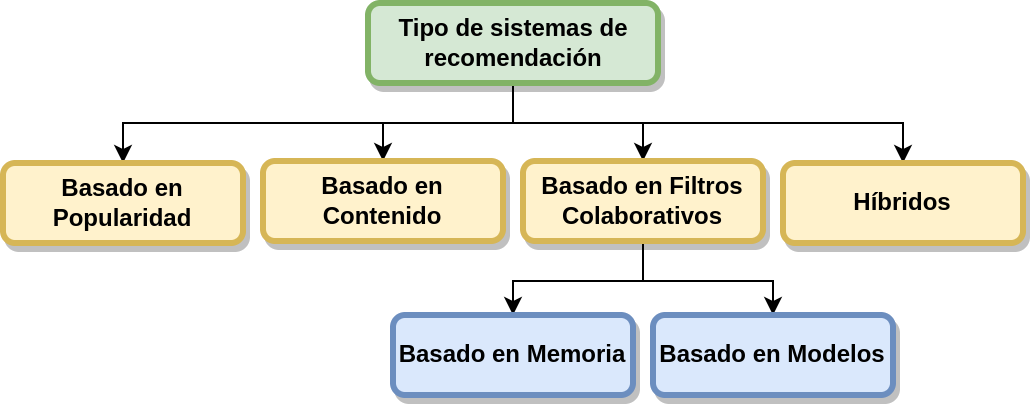
\includegraphics[width=12cm]{./images/clasificacion-sis-rec.png}
	\caption{Clasificación de tipos de sistemas de recomendaciones.}
\end{figure}

\subsection{Basados en Popularidad} 

Este tipo de recomendadores toman alguna característica de popularidad de los items en cuestión, como puede ser: cantidad de vistas, cantidad de compras, cantidad de reviews positivos, o una conjunción de estos. Luego busca el top K de los items mas populares. Si bien este tipo de recomendaciones tiene buenos resultandos para usuarios nuevos, sus recomendaciones no tienen en cuenta las preferencias de cada usuario particular, debido a que se basan en estadísticas comunes a todos los usuarios. Por esta cuestión, muchas veces no son considerados sistemas de recomendación perse.

\subsection{Basados en Contenido}

Este tipo de recomendador necesita un trabajo previo de ingeniería de features sobre los items, donde se busca definir que features son los mas significativos para la tarea en cuestión, y cual es el grado de adecuación de cada items a los features definidos. Por otro lado, es necesario registrar las interacciones de los usuarios. Dadas estas interacciones, se puede definir el grado de preferencia de los usuarios a cada feature definido para los items. Con esta información es posible encontrar tanto items como usuarios similares y realizar recomendaciones del tipo:

\begin{itemize}
\item Dado el usuario A, el cual tiene preferencia por el item X, también podría tener preferencia por el item Y, por ser muy cercano o similar al item X.
\item Dos usuarios A y B cercanos o similares tendrán preferencias similares. De esta forma es posible recomendar item consumidos por el usuario A al usuario B y vise versa. 
\end{itemize}
	
La principal desventaja de este enfoque reside en que, es necesario realizar ingeniería de features para encontrar los features que produzcan las mejores recomendaciones. El modelo no encuentra estos features automáticamente, sino que deben ser definidos de antemano manualmente. Como ventaja, si se encuentra los features correctos se pueden lograr muy buenas recomendaciones.
		
\subsection{Basados en Filtrado Colaborativos} 

Estos modelos, a diferencia de los modelos basados en contenido, no requiriere ingeniería de features, lo que los hace mas simples de implementar, ya que únicamente es necesario registrar las interacciones de los usuarios para con los items. Ejemplos interacciones podrían ser:

\begin{itemize}
	\item El usuario A visualizo el item X el dia 2 de marzo de 2022.
	\item El usuario A compro el item X el dia 10 de marzo de 2022.
	\item El usuario A califico al item X con 5 puntos el dia 25 de marzo de 2022.
\end{itemize}

Ambos tipo de modelos, basados en contenido y filtros colaborativos, personalizan sus recomendaciones. 
Es decir, ajustan las recomendaciones a cada usuario particular, en base a sus preferencias. Ademas, ambos permiten encontrar usuarios e items similares y recomendar items entre usuarios similares.

Por otro lado, un ventaja del modelo de filtros colaborativos es que descubre un espacio latente de soluciones sin necesidad de recolectar datos y definir features en forma manual. Esto podría llevar a una solución sesgada ya que la selección de features no esta basada en datos, sino en el juicio experto del científico de datos. 
No todo son rosas con estos modelos, ya que sufren un problema llamado \textit{Cold start} o arranque en frio. Si pensamos en una solución donde alimentamos al modelo con una ventana de interacciones usuario-item filtrando los últimos N meses, tendremos las siguiente situaciones:

\begin{itemize}
	\item Usuarios nuevos: Los usuarios nuevos no tendrán interacciones. Por lo tanto, este modelo no podrá realizar ninguna recomendación. En general, se establece un mínimo de interacciones para que el modelo pueda realizar recomendaciones acertadas, ya que con pocas interacciones no podrá realizar buenas recomendaciones.
	\item Usuarios con pocas interacciones: Por otro lado, tenemos a los usuarios que tienen una baja \textit{velocity} en cuando a interacciones con el sistema o aplicación. Si pensamos en un \textit{e-commerce}, hay usuario que compran con mucha frecuencia y otros que compran muy de vez en cuando. Estos últimos, en general tendrán pocas interacciones pudiendo caer por debajo del umbral mínimo que requiere el modelo. De esta forma, tendremos usuarios que quedaran fuera del modelo actual.
	\item Usuarios con muchas interacciones: Este es el caso ideal, donde el usuario tiene una gran cantidad de interacciones con item. Para estos usuarios, el modelo podrá ofrecer mejores recomendaciones, ya que cuanto mas interacciones se tengan, el modelo se ajusta con mas facilidad a sus preferencia.


\end{itemize}

\clearpage
\subsection{Modelos Híbridos}

Son aquellos modelos que combinan mas de una técnica de recomendación, también llamados ensambles de modelos. En general, lo mas común es combinar modelos de recomendación por popularidad, basados en contenido y filtros colaborativos. De esta forma, cuando los usuarios caen por debajo del umbral de interacciones necesarias por el modelo de filtro colaborativos, se utiliza un modelo basado en contenido, popularidad, o alguno otro modelo que no requiere de interacciones del usuario para realizar sus recomendaciones.

\subsection{Categorías dentro de los modelos basados en filtros colaborativos} 

Dentro de los sistemas de recomendación basados en filtros colaborativos, tenemos dos sub-clasificaciones referidas a la forma en la que se realizan las predicciones:

 \subsubsection{Basados en Memoria} 
 
 Este tipo de modelos mantiene sus datos en memoria. Se recorren todos los datos (\textit{full scan}) cada vez que se necesita realizar un inferencia o predicción (fijando un número de vecinos a comparar). Un ejemplo de estos modelos es el algoritmo de k vecinos cercanos (\textit{KNN}), el cual mantiene una matriz rala de distancias en memoria, la cual se recorre completamente para comparar las distancias entre filas o columnas, usando alguna medida de distancia como puede ser la distancia coseno, coseno ajustada, \textit{manhattan}, etc..
 Para mitigar el problema de búsqueda exhaustiva, se puede utilizar una cache para realizar estas búsquedas una única vez. Otro problema es su limitación al tamaño máximo de la memoria con la que se cuenta, es decir, que el tamaño de la matriz depende de la memoria máxima disponible. Esto puede mitigarse utilizando implementaciones de matrices esparzas, las cuales comprimen los datos en memoria guardando unicamente las celdas que tiene datos. Ademas, es posible utilizar un cache que mantenga en memoria las búsqueda mas frecuentes y baje a almacenamiento secundario las menos frecuentes. Todos estos problemas de \textit{performance} y uso de recursos se deben a que \textit{KNN} no reduce la dimensionalidad de los datos, como si lo hacen varias implementaciones basadas en \textit{embeddings}, auto-encoder, redes neuronales etc.., donde lo que se buscan es encontrar una representación mas compacta de los items y usuarios sin perder información. Mas allá de tener que lidiar con estos problemas de escalabilidad, los resultados obtenidos por estos modelos no están muy alejados de aquellos que se encuentran en el estado del arte. Puede recomendarse su uso cuando tenemos un dominio reducido, dada su simplicidad. 

 \subsubsection{Basados en Modelos}
 
Algunos ejemplos de estos modelos son los clasificadores bayesianos, redes neuronales, algoritmos genéticos, sistemas difusos y la técnica de descomposición matricial (\textit{SVD}). Estos modelos en general buscan directa o indirectamente reducir la dimensionalidad de los datos. De esta forma, es posible utilizarlos en dominios con una gran cantidad de datos.

\clearpage
\section{Descripción del problema y motivación}

Con este trabajo se busca contestar las siguientes preguntas:

\subsection{¿Los modelos basado en filtro colaborativos que utilizan técnicos de Deep Learning, obtienen mejores resultados?}

La idea detrás de esta pregunta es realizar benchmarks sobre distintos modelos del estado de arte basados en Deep Learning o no, utilizando el mismo set de datos y las mismas métricas. De esta forma, se busca comprender cual es la diferencia en \textit{performance} entre los modelos seleccionados. Por otro lado, se busca comprender cuando es mas adecuado utilizar cada enfoque. Como ya se comentó en el apartado de introducción, hay modelos que están mas limitados que otros según el número de recursos de \textit{hardware} o interacciones con los que se cuenta.

\subsection{¿Cuáles son las ventajas y desventajas de cada enfoque a la hora de aplicar estas técnicas?}

Esta pregunta se refiere a comprender cuando es conveniente aplicar una técnica u otra teniendo en cuenta las ventajas y desventajas de cada enfoque y modelo.

\subsection{¿Cómo se puede solucionar el problema de \textit{cold-start} que sufre el enfoque de recomendación basado en filtros colaborativos?} (Tesis)

Como ya se comentó en la introducción, los modelos de filtro colaborativos necesitan un número mínimo de interacciones usuario-item para poder operar y producir recomendaciones aceptables. La propuesta es explorar enfoques que permiten lidiar con este problema. Uno de los enfoques más comunes es utilizar ensambles de modelos basados en filtros colaborativos con otros modelo basados en contenidos. Estos ensambles puede diferir en sus técnicas dependiendo del dominio de los datos.

\section{Objetivos}

Como primer objetivos, se pretender comprender cuales son los fundamentos teóricos sobre los que se apoya cada técnica aplicada y bajo que escenarios puede ser conveniente aplicarlas. Por otro lado, se intenta determinar cual es la diferencia en performance de cada técnica aplicada sobre el mismo set de datos, midiendo su performance utilizando las mismas métricas. ¿Obtenemos diferencias significativas?

Como segundo objetivo se busca proponer nuevas técnicas y/o explorar técnicas existentes que permite lidiar o solucionar el problema de cold start que sufren los sistemas de recomendación basados en filtros colaborativos (Tesis).

Finalmente, se compararan esta técnicas mediante el \textit{benchmark} propuesto para compara como se comporta cada modelos ante usuarios con escasas o ninguna interacción en el set de datos propuesto.

\chapter{Materiales y Métodos}

\section{Datos} 

Para realizar este trabajo se selecciono el dominio del cine, ya que existen conjuntos de datos bien definidor y actualizados. 
Estos \textit{datasets} en general están pensados para probar modelos de recomendación. Por otro lado, es el dominio clásico en papers y literatura de sistemas de recomendación en general.

Dada la propuesta de este trabajo, es necesario contar con datos de interacciones de usuarios con items(Películas en este caso). Ademas, dado que se busca solucionar el problema de \textit{cold start} para el enfoque de filtros colaborativos, se necesitara contar con otro enfoque de recomendación, el cual posiblemente pueda ser basado en contenido. Por esta cuestión, necesitamos contar con features completos y consistentes para los items(Películas).

Dadas estas necesidades se decidió utilizar los siguientes \textit{datasets}:


\subsection{\href{https://grouplens.org/datasets/movielens/25m/}{MovieLens 25M Dataset}}

Este \textit{dataset} prácticamente no tiene features para los items(Películas), pero si tiene las calificaciones realizadas 
por los usuarios. También cuenta con un conjunto de \textit{tags} o palabras clave cargadas por los usuarios para cada 
item(Película). Otro punto importante, es que todos los usuarios tienen al menos 20 interacciones, lo cual asegura
no tener problemas de baja performance por falta de interacciones. 
De esta forma, este \textit{dataset} sera muy util para entrenar modelos de recomendación basados en filtros colaborativos
y ademas cuenta con columnas extras como \textit{tags}, que serán útiles a la hora de entrenar modelos basados en contenido.
Por ultimo, este \textit{dataset} contiene 25.000.095 calificaciones, 1.093.360 tags y 62.423 películas. Estos datos fueron registrados por 162.541 usuarios entre el 9 de enero de 1995 y el 21 de noviembre de 2019. Las columnas que se utilizaron son las siguientes:

\begin{itemize}
	\item userId 
	\item movieId
	\item timestamp: Fecha en la cual el usuario califico el item(movieId). Es un string de formato año-mes. Existen valores entre 1997-09 y 2019-11 inclusive.
	\item rating:    Calificación. Es un valor discreto numérico: 0.5, 1, 1.5, 2, 2.5, 3, 3.5, 4, 4.5, 5.
	\item tags:      Lista de palabras definidas por cada usuario para una película. Se cuenta con los tags a nivel usuario-película.
	\item timestamp
\end{itemize}


\subsection{\href{https://www.kaggle.com/datasets/rounakbanik/the-movies-dataset?select=movies_metadata.csv}{TMDB Movie Dataset}}

Este \textit{dataset} no tiene calificaciones personalizadas de los items como sucede con el \textit{dataset} anterior, 
pero tiene varios features referentes a películas que pueden ser muy útiles para modelos basados en contenido e inclusive
modelos híbridos, los cuales se busca explorar en el trabajo de tesis. Contiene datos de 5.000 películas con los siguientes campos:

\begin{itemize}
	\item imdb\_id: identificador univoco en la base de datos de imdb.
	\item title y original\_title
	\item release\_date: Fecha de estreno.
	\item status: Define si la película fue estrenada o esta en desarrollo.
	\item overview:	Sinopsis de la película.
	\item poster\_path: Url de imagen de portada.
	\item languages: Lenguaje original y doblaje.
	\item genres: Géneros.
	\item adult: Es para adultos?
	\item popularity: Indice de popularidad.
	\item vote average/count: Cantidad y media de votos.
	\item keywords/tagline: \textit{tags}.
	\item budget/revenue: Presupuesto.
	\item production companies/countries: Países y compañía que produjeron la película. 
	\item homepage: Sitio.
\end{itemize}


\subsection{Preprocesamiento}

Como parte inicial de la etapa de pre-procesamiento de datos se utilizo una base de datos \textit{MongoDB}. Se utilizo \textit{MongoDB} y no \textit{Pandas} debido a que pandas requiere cargar todo el \textit{dataset} en memoria. Si bien este problema se puede lidiar aumentado el tamaño de la memoria \textit{Swap}(Linux) o la memoria virtual(Windows), puede ocasionar caídas de procesos y lentitudes innecesarias. En este caso, se selecciono una base de datos de tipo documento, la cual no necesita cargar todos los datos en memoria y por otro lado, existe la posibilidad de escalar la base de datos a mas nodos en caso de ser necesario.
Ambos \textit{datasets} contienen varios archivos \textit{csv} los cuales vamos a llamar \textit{tablas}, de los cuales se utilizaron los siguientes:

\begin{itemize}
	\item movie\_metadata: Pertenece al \textit{dataset} \textit{TMDB}. Es la fuente de verdad de las cual se toman columnas con datos referentes a películas.
	\item tags: Pertenece al \textit{dataset} \textit{Movie Lens}. De esta tabla se tomaron los tags o palabras clave dadas de alta por los usuarios por cada película.
	\item ratings: Pertenece al \textit{dataset} \textit{Movie Lens}. De esta tabla se tomaron las calificaciones de los usuario para las películas que fueron calificadas.
\end{itemize}

De esta forma, primero se realizo un merge o join de las tabla ratings y tags por las columnas user\_id y movie\_id,
 ya que tenemos dos columnas que representan interacciones de usuarios: 

\begin{itemize}
	\item rating: Pertenece a la tabla ratings.
	\item tags: Pertenece a la tabla tags.
\end{itemize}

En segundo lugar se hizo merge entre las tablas ratings\_tags\_v1 y movie\_metadata utilizando la columnas imdb\_id, la cual es identificador único de las películas en ambas tablas.

Finalmente se termino con dos tablas como resultado:

\begin{itemize}
	\item movies\_v4.csv: Contente toda la información de las películas, incluidos todos los tags cargados por los usuarios que calificaron un película.
	\item ratings\_tags\_v1.csv: Contiene tanto las calificaciones como los tags para cada usuario y película. 
\end{itemize}

\subsubsection{Tabla de interacciones}

La tabla ratings\_tags\_v1 tiene datos a nivel interacción usuario-item. De esta forma a nivel usuario-item se cuenta con la calificación de la película realizada por el usuario, ademas de los tags que el usuario cargo para esa películas. Estos tags no son mas que una lista de palabras que son representativas de la película en cuestión. 
Por ejemplo, para la película \textit{Toy Story} deberíamos tener palabras referente a la misma como: boss, woody, 
animation, 3d, etc.. Finalmente, contamos con la fecha en la cual se realizaron esta interacciones. Se entiende 
que la calificación y los tags se ingresaron en el mismo momento.


La definición de la tabla es la siguiente:

\begin{itemize}
	\item user\_id:  Existen 13.281 usuarios.
	\item movie\_id: Existen 33.444 películas.
	\item timestamp: Fecha en la cual el usuario califico el item(movie\_id). Es un string de formato año-mes. Existen valores entre 1997-09 y 2019-11 inclusive.
	\item rating:    Calificación. Es un valor discreto numérico: 0.5, 1, 1.5, 2, 2.5, 3, 3.5, 4, 4.5, 5.
	\item tags:      Lista de palabras definidas por cada usuario para una película. Se cuenta con los tags a nivel usuario-película.
\end{itemize}


\clearpage
\subsubsection*{Tablas de metadata de películas}

La tabla movies\_v4 cuenta con información de cada película seleccionada de ambos \textit{datasets}. 

\begin{itemize}
	\item title: 	Título de la película.
	\item native\_languaje: Lenguaje original en el cual fue filmada la película.
	\item genres:  	Ambos \textit{dataset} cuentan con una lista de géneros a los adiare la película.
	\item overview:	Sinopsis de la película.
	\item poster:	Enlaces al detalle de la película en imdb y TMDB. Estos enlaces
					permiten hace join con mas datos que se encuentren en la descripción de estos
			 		sitios. En este trabajo solo se utilizara la imagen de la tapa de las película
					a modo de visualización.
	\item release: 		Fecha de lanzamiento.
	\item budget: 		Presupuesto destinado para la realización el film.
	\item popularity: 	Popularidad.
	\item vote\_count: 	Cantidad de votos por película.
	\item vote\_mean: 	Cantidad media de votos por película.
	\item tags:         Son los tags cargados por todos los usuarios que interactuaron con la película. 
						Es la mismas información que tenemos en la tabla de interacción pero ahora a nivel item.
\end{itemize}

\subsubsection*{Valores faltantes}

Una vez generadas ambas tablas se procedió a buscar missing values. A continuación en la tabla \ref{table:tab} 
se pueden ver las columnas con missing values:
\begin{table}[h!]
\centering
\footnotesize
\begin{tabular}{lrrrrrr}
\hline
Columna &  Porcentaje de missing values \\
\hline
   	budget     &  70      \\
   	poster     &  0.00085 \\
   	release    &  0.0085  \\
	popularity &  0.00085 \\
	vote\_mean  &  4.8     \\
	vote\_count &  4.6     \\
\hline
\end{tabular}
\caption{Missing values en la tabla movies\_v4.}
\label{table:tab}
\end{table}

Luego se removieron las filas de la tabla para aquellas columnas del reporte anterior que tuvieran hasta 6 \% de valores faltantes. A continuación se removió la columna budget por tener un porcentaje muy alto de valores faltantes lo que la volvió inutilizable. Por otro lado, la tabla ratings\_tags\_v1 no se modifico, ya que no tenia valores faltantes en ninguna de sus columnas.


\clearpage
\section{Análisis exploratorio}


\subsection{Variable Rating}


En este análisis exploratorio analizaremos datos relevantes al problema de predicción de calificaciones de items por parte de los usuarios. Dentro de este análisis, la variable ratings o calificación es una de estas variables relevantes.

A continuación se puede apreciar una diagrama de barras el cual describe la frecuencia con la que los usuarios califican un item segmentada por cada valor posible de calificación:


\begin{figure}[h!]
	\centering
	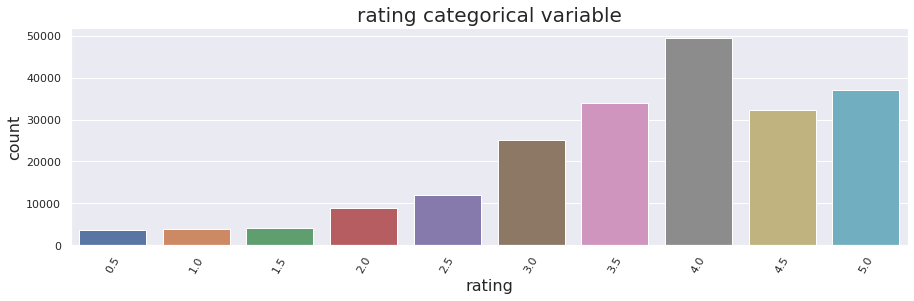
\includegraphics[width=15cm]{./images/rating-barplot.png}
	\caption{Este diagrama de barras expone la frecuencia o cantidad de observaciones para cada valor discreto de puntuación o rating.}
	\label{fig:ratingsBarPlot}
\end{figure}

En la figura ~\ref{fig:ratingsBarPlot} se puede visualizar que 4 puntos es la calificación con la mayor frecuencia(moda), seguido de 5 puntos y luego 3.5 puntos. Por otro lado, se debe tener en cuenta que estas calificaciones provienen de todo los usuarios. Cada usuario tiene una forma propia de calificar, algunos tienden a calificar de forma optimista, puntuando con valores altos, y otros por el contrario, son mas pesimistas y tienden a puntuar con calificaciones bajas. Este es un comportamiento conocido en el ámbito de sistemas de recomendación. Se debe tener en cuenta que un 3.5 para un usuario podría ser un 4.5 para otro. Por otro lado, se aprecia que en general se tiende a puntuar valores a partir de 3 punto en adelante, habiendo muy pocas observaciones para puntuaciones menores a 2 puntos.

\clearpage

Para analizar en mas detalle la variable rating, veamos a continuación histograma y boxplot respectivamente:

\begin{center}
\end{center}

\begin{figure}[h!]
	\centering
	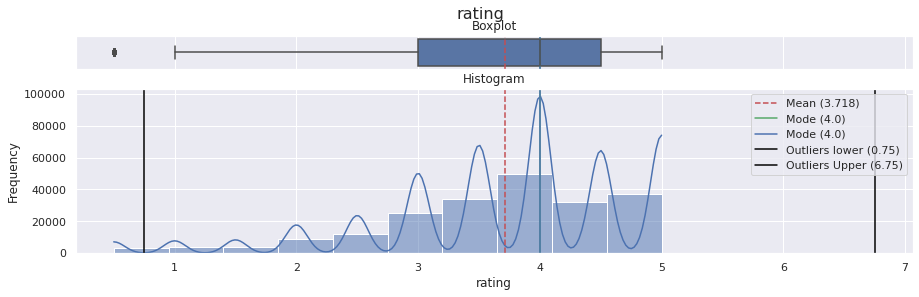
\includegraphics[width=15cm]{./images/rating-boxplot-histplot.png}
	\caption{Histograma y Boxplot de la variable rating. Los ratings son las calificaciones realizadas por los usuario para cada item o película.}
	\label{fig:ratingsHistPlot}
\end{figure}

En la figura ~\ref{fig:ratingsHistPlot} se aprecia claramente que esta variable es categórica y no numérica, debido a los picos con distintos niveles en en el histograma. Esta variable tiene valores discretos entre 0.5 y 5 con un paso de 0.5. De esta forma, contamos con 10 valores discreto de tipo real, siendo claramente una variable categórica. Nuevamente vemos algo parecido en diagrama de barras, el 50\% de las observaciones se encuentran entre los cuantiles Q1 y Q3 con 3 y 4.5 puntos (Rango inter-cuantil). La mediana(Cuantil Q2) esta claramente sobre los 4 puntos, coincidiendo con la moda. La media se encuentra en los 3.5 puntos a izquierda de la mediana, debido a que tenemos puntos con frecuencia considerables a izquierda que mueven a la media en esa dirección.
Por otro lado, tenemos valores atípicos en el extreme izquierdo en los 0.5 puntos. Esto se debe a que esta puntuación esta muy alejada del centro de los datos, el cual encuentra entre el cuantiles Q1 y Q3, donde tenemos el 50\% las calificaciones con major probabilidad de ocurrencia. No se encuentran valores atípicos por sobre el máximo.
Se puede apreciar un sesgo a izquierda, ya que existe mayor separación o dispersión de las observaciones entre Q1 y Q2 que entre Q2 y Q3. De esta forma, ambos intervalos conservan su 25\% de las observaciones pero hay menor dispersión entre Q2 y Q3.


\clearpage
A continuación segmentemos el anterior histograma por año:

\begin{figure}[h!]
	\centering
	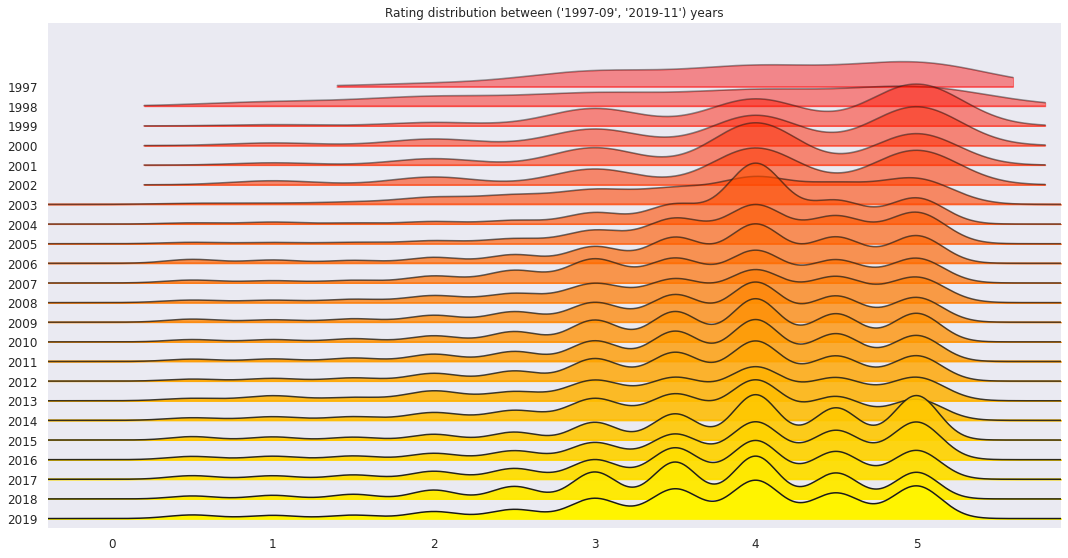
\includegraphics[width=15cm]{./images/rating-by-year.png}
	\caption{Histograma de calificaciones segmentado por año.}
	\label{fig:ratingsYearHistPlot}
\end{figure}


En la figura ~\ref{fig:ratingsYearHistPlot} inicialmente vemos que en los años 1997, 1998 y 2003 la curva tiende a ser mas lineal. Esto indica que la forma de calificar es mas dispersa, es decir, no se encuentra un perfil de puntuación claro por parte de los usuarios, en que item es un 4 o un 5 por ejemplo. Entre 1999 y 2022 vemos que las puntuaciones 3, 4 y 5 toman mayor importancia siendo estas las mas utilizadas. Es decir, los usuarios realizan en su mayoría puntuaciones en esos tres niveles. La mayor frecuencia se puede ver claramente en 4 puntos en el año 2004, donde fue prácticamente la mas utilidades decayendo los 3 y 5 puntos en linea a años anteriores. A partir del año 2005 se nota un aumento cada ves mas demarcado en los niveles de puntuaciones entre los 3 y 5 puntos donde los usuarios cada ves usan mas lo niveles 3.5 y 4.5. Debemos tener en cuenta que el aumento en los niveles de puntuación con el tiempo probablemente sea debido a un aumento año a año en la base de usuarios de \textit{Movie Lens} y tal vez también sea el motivo por el cual en los primeros años vemos mucho dispersion en las puntuaciones.

\clearpage

\subsection{Correlaciones}

Para realizar un analizar de correlación sobre todas la variables, se realizo un merge/join de las tabla movies y interactions, incluyendo solamente las columna numéricas. A continuación podemos visualizar un diagrama de correlación de Pearson de las mismas:

\begin{figure}[h!]
	\centering
	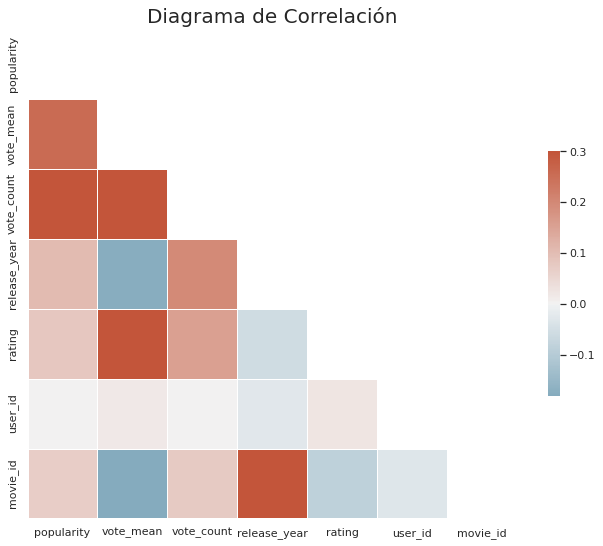
\includegraphics[width=9cm]{./images/Correlations.png}
	\caption{Diagrama de correlación de Person aplicado a todas las variables numéricas resultado del merge entre las tablas movies y interactions.}
	\label{fig:correlationPlot}
\end{figure}	


En la figura ~\ref{fig:correlationPlot} se aprecia de las variables \textit{Cantidad/Media de votos} y \textit{Popularidad} tiene alta correlación debido a que las películas mas votadas en general son las mas populares. 
las variables \textit{Cantidad} y \textit{media de votos} están altamente correlacionadas, ya que la media se calcula en base a la variable \textit{Cantidad de votos}. Por otro lado, también es de esperar que las \textit{calificaciones} y la \textit{media de los votos} este correlacionadas, ya que a medida de aumenta la \textit{media de los votos} tenemos calificaciones mas altas. Se encuentra una alta correlación entre la variable que identifica a una película y la \textit{Fecha de estreno}. Esto se debe a que al momento de estrenarse una película, días después a mas tardar, se da de alta la película en el sitio de \textit{Movie Lens}. Esto también nos dice que los ids son secuenciales.
Las correlaciones en general son muy bajas llegando a 0.3 como máximo. Esto es una buena señal, ya que ayuda a diminuir el fenómeno de colinealidad de las variables. Las variables que son combinaciones lineales de otras variables puede producir que los modelos de \textit{Machine Learning} sobre-ajusten a los datos de entrenamiento. 
Las variables \textit{media de votos} y \textit{id de película} tienen una correlación negativa muy baja. En algún sentido nos dice que algunas películas mas nuevas tiende a tener una media de votos menor. Lo mismo sucede entre las variables \textit{rating} y \textit{id de película} en menor medida. Ambas con correlaciones negativas pero muy bajas.


Si bien, en esta primera entrega no se están utilizando otras variables distintas a \textit{id de usuario}, \textit{id de película} y \textit{rating}, es de interés analizar las variables correspondiente a features de películas, ya que en el siguiente entrega (tesis) se planea implementar modelos de recomendación híbridos, los cuales son ensambles de sistemas de recomendación basados en contenido y colaborativos.

\subsection{Variables de tipo texto}

Las variables de tipo texto son muy útiles para genera \textit{embeddings}, los cuales se puede sumar o promediar, generando representaciones compactas de items a recomendar. Luego es posible utilizar estas representaciones para agrupar items según su sinopsis, \textit{tags}, título y otras variables como pueden ser popularidad, año de estreno, votos, \textit{ratings}, etc...

A continuación se puede visualizar la frecuencia de aparición de cada palabra en cada uno de los campos de tipo texto. Cuanto mayor tamaño tenga la palabra mayor frecuencia de aparición tendrá.

\begin{description}
	\item[Tags]
\end{description}

Cada usuario puede asociar tags o palabras clase a una película. Un tags es una palabra o frase corta que identifica o describe una película. Es una forma simple de clusterizar, ya que los usuarios en general describen categorías como animación 3d, cual es el director, una frase que describe algún tipo de categoría o algo relevante en el contenido de la misma. 

\begin{figure}[h!]
	\centering
	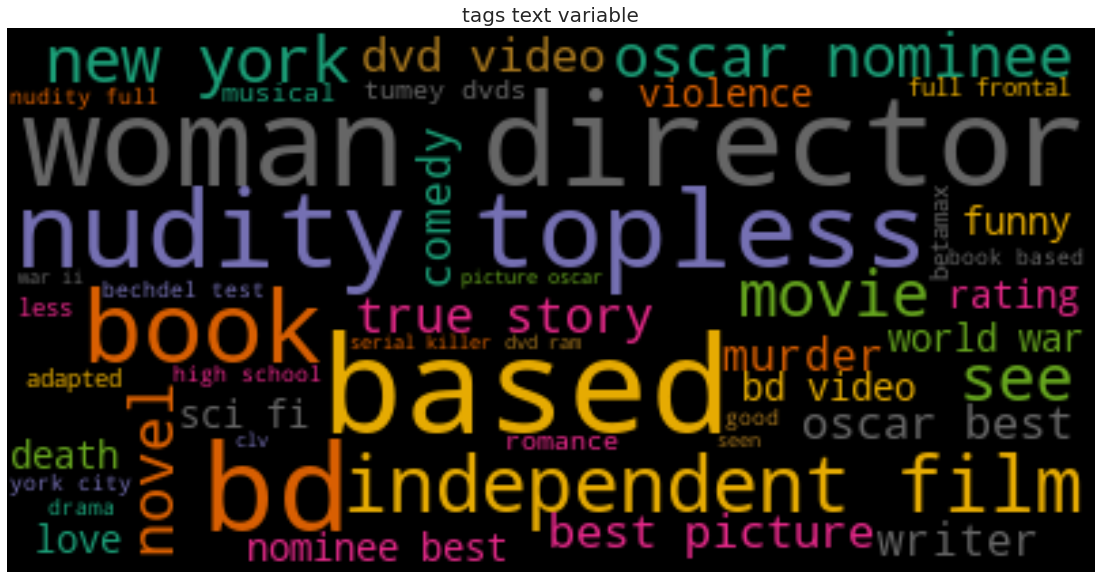
\includegraphics[width=9cm]{./images/Cloud-tags.png}
	\caption{Frecuencia de frases encontradas en la variable \textit{Tags}. El tamaño de cada frase representan la cantidad de apariciones de la misma.}
	\label{fig:tagsCloud}
\end{figure}	


En la figura ~\ref{fig:tagsCloud} las palabra \textit{based} (basada/o en...), \textit{Book}, \textit{Bd}, \textit{Director}, \textit{Nudity}, \textit{Topless}, \textit{Independent}, \textit{Film}, son aquella palabras mas utilizadas en los tags que cargan los usuarios para cada película. Otras palabras de menor frecuencia: \textit{Movie}, \textit{Morder}, \textit{Novel}, \textit{Funny}, \textit{Oscar nominee}, \textit{Violent}, \textit{World war}, \textit{True story}.


\clearpage

\begin{description}
	\item[Overview]
\end{description}

La variable \textit{overview} es la sinopsis de la película. Esta describe brevemente el contenido de la misma, sin revelar su desenlace.

\begin{figure}[h!]
	\centering
	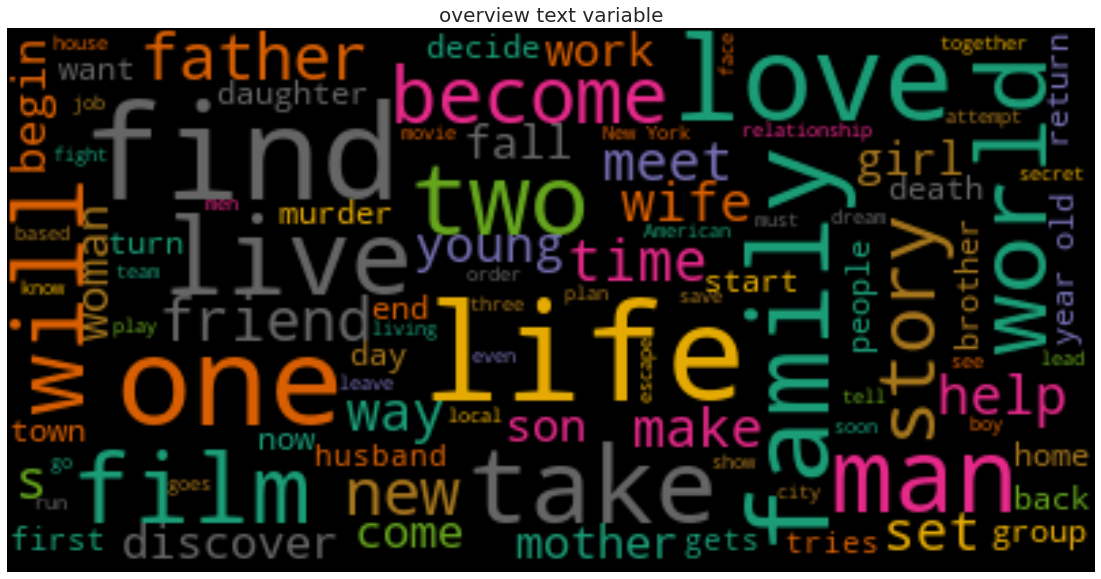
\includegraphics[width=9cm]{./images/Cloud-Overview.png}
	\caption{Frecuencia de palabras encontradas en la variable \textit{Overview}. El tamaño de cada palabra representan la cantidad de apariciones de la misma.}
	\label{fig:tagsCloud}
\end{figure}	


En la figura ~\ref{fig:tagsCloud} podemos visualizar las siguientes palabra con mayor frecuencia: \textit{Find}, \textit{Live}, \textit{Love}, \textit{Wife}, \textit{One}, \textit{Man}, \textit{Film}, \textit{Become}, \textit{Family}, \textit{Story}, \textit{World}, \textit{Work}, \textit{Father}, \textit{New}, \textit{Friend} y \textit{Story}. Se aprecia una diferencia notoria entre las variables tags y overview. La variable tags parece categorizar las películas desde distintas perspectivas. Por otro lado, la variable overview contiene palabras que son mas utilizadas en la descripción de la misma. A simple vista, los clústeres(\textit{Embeddings}) que pudieran generarse utilizando esta variable, podrían ser mas específicos que aquellos clusters generados a partir de la variable tags.


\begin{description}
	\item[Title]
\end{description}

\begin{figure}[h!]
	\centering
	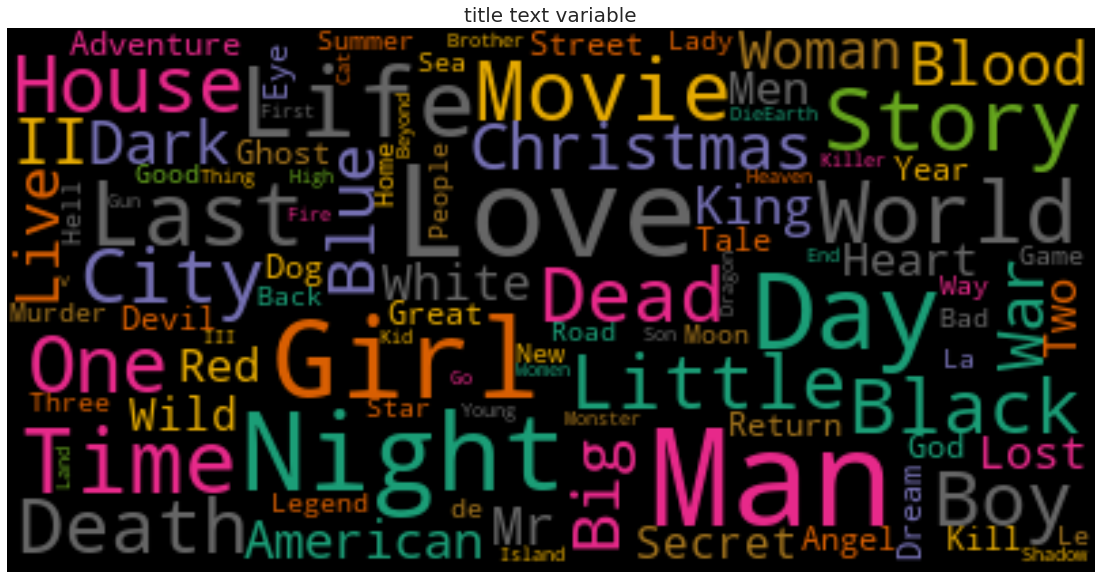
\includegraphics[width=9cm]{./images/Cloud-Title.png}
	\caption{Frecuencia de palabras encontradas en la variable \textit{Title}. El tamaño de cada palabra representan la cantidad de apariciones de la misma.}
	\label{fig:titleCloud}
\end{figure}	


En la figura ~\ref{fig:tagsCloud} podemos visualizar las siguientes palabras con mayor frecuencia: \textit{Girl}, \textit{Man}, \textit{Day}, \textit{Dead}, \textit{Movie}, \textit{Time}, \textit{Night}, \textit{Life}, \textit{House}, \textit{Dark}, \textit{II}, \textit{Blood}, \textit{Christmas}, \textit{World}, \textit{War}, \textit{Black}, \textit{Boy}, \textit{Blue}, \textit{One} y \textit{King}. A simple vista, una clusterización realizada con esta variable puede ser mas general que la lograda con la variable \textit{Overview}, pero en menos general que la variable \textit{Tags}. En trabajos posteriores se realizaran experimentos para ver resultado en este sentido.


\clearpage

\subsection{Análisis de Componente Principales}

En esta sección describe el análisis de componentes principales realizado sobre las variable numéricas resultado del merge de las tablas movies y interactions.

\begin{description}
	\item[Varianza Explicada]
\end{description}

Las componentes principales son las variables resultado del algoritmo PCA. Estas nuevas variables tiene la particularidad de ser ortogonales entre si, lo cual indica que no tienen correlación alguna. Ademas de esto, desde la primera hasta a la última variable la acumulación de varianza es decrecientes, es decir, que la primera componente tiene major varianza y la última la menor posible. 


\begin{figure}[h!]
	\centering
	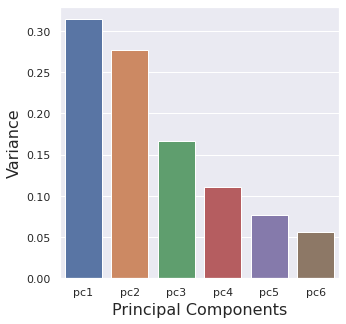
\includegraphics[width=8cm]{./images/PCA-Variance.png}
	\caption{Este diagrama de barras describe el grado de variabilidad o varianza explicada por cada componente principal resultado del algoritmo PCA.}
	\label{fig:explainedVariancePlot}
\end{figure}


\begin{description}
	\item[Varianza]
\end{description}
\begin{itemize}
	\item pc1: $31$ \%
	\item pc2: $28$\%
	\item pc3: $16$ \%
	\item pc4: $11$ \%
	\item pc5: $7$ \%
	\item pc6: $5$ \%
\end{itemize}

Inicialmente podemos apreciar en la figura ~\ref{fig:explainedVariancePlot} que toda las componente tiene niveles de variabilidad o varianza explicada muy bajos, donde la primera componente llega solamente al $31$ \%. Esto indica que el grado de correlación de las variables es muy bajo. Usando el criterio del bastón roto podríamos seleccionar las 3 primeras variables, ya que son las que acumulan mayor varianza. Tengamos en cuenta que el análisis por componentes principales es un análisis lineal. Es decir que, tiene encuentra unicamente correlaciones lineales. De esta forma este método puede estar perdiendo de vista correlaciones no lineales mas complejas donde podríamos encontrar un mayor grado de correlación. Las 3 primeras componentes acumulan un grado de variabilidad 85 \%.


\begin{description}
	\item[Cargas o Loadings]
\end{description}

Por otro lado las componentes principales son combinaciones lineales de las variable originales. Luego, las carga o loadings son los coeficientes utilizados para transformar las variables originales en las componentes principales mediante combinaciones lineales.

De esta forma, los coeficientes definen una medida de correlación o grado de aporte de cada variable original a una componente principal.

A continuación se pueden visualizar las cargas o loadings:

\begin{table}[h!]
	\centering
	\begin{tabular}{lrrrrrr}
			\toprule Variable & PC1    &  PC2  & PC3    \\
			\midrule Popularity  &0.79   & -0.09 & -0.003  \\
					Vote Mean & 0.55   & -0.55 & -0.03      \\
					Vote Count & 0.88   & -0.11 & -0.0002\\
					Release Year & 0.33   &  0.8  &  0.045\\
					User ID & -0.006 & -0.08 &  0.99    \\
					Movie ID & 0.24   &  0.8  &  0.04 \\
			\bottomrule
	\end{tabular}

	\caption{Coeficientes de componentes principales vs. variable originales. Cada uno de estos valores representan el grado de correlación o aporte de cada variable original a cada componente principal.}

	\label{fig:loadingsTable}
\end{table}


En la tabla ~\ref{fig:loadingsTable} vemos que \textit{Vote Count(88\%)} y \textit{Popularity(80\%)} tiene una correlación positiva muy alta sobre la componente $PC1$. Lo mismo sucede con la \textit{Vote Mean(55\%)} en menor medida. Entre dos observaciones con distintos valores de popularidad, la que tenga un valor mas alto aportara a esta componente($PC1$) que a las otra ($PC2$ y $PC3$). También vemos que las variable \textit{Release Year(Año de estreno)} y \textit{Movie ID} tienen un aporte considerable pero mas bajo del 33\% y 24\% respectivamente, sobre la componente $PC1$. La variable \textit{User ID} no tiene aporte alguno sobre componente $PC1$. Las variables que mas aportan a la componente $PC2$ son \textit{Vote Mean(55\%)} y \textit{Vote Count(11\%} respectivamente. Este aporte es negativo, esto quiere decir que un aumento en los niveles de esta variable significa una disposición en esta componente. La variable \textit{Release Year(Año de estreno)} tiene el aporte positivo mas alto sobre la componente $PC2$ siendo del 80 \%. Para la componente $PC3$ vemos que las variables que mas aportan a un campo en la misma son \textit{User ID(99\%)} y \textit{Release Year (45\%)} respectivamente, ambos positivos. Veamos que un aumento en la variable \text{User ID)} produce un aumento casi en una unidad sobre el coeficiente, pero \textit{Release Year} es la mitad en relación. De este forma, la componente $PC1$ podríamos nombrarla \textit{Nivel de popularidad o conocimiento general de una película}. La componente $PC2$ en algún sentida mide lo contrario a la popularidad. Es un indicador del \textit{Nivel Underground para nuevos estrenos} de un film.  La componente $PC3$ es mas difícil de nombrar pero podría llamarse: \textit{Grado newbie de un usuario}.


\begin{description}
	\item[Biplot]
\end{description}
\begin{figure}[h!]
	\centering
	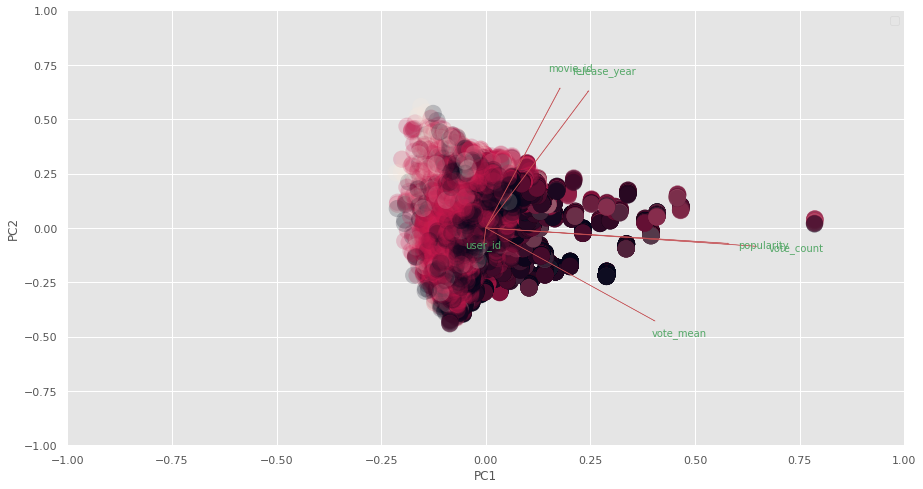
\includegraphics[width=15cm]{./images/PCA-biplot.png}
	\caption{En este diagrama se pueden visualizar los valores de las variables originales coloreados en color roja, negro y gris correspondientes a tres segmentos de calificaciones: $>2$, entre $2$ y $3.5$ y $>4$. También se pueden apreciar los vectores correspondientes a las variables originales.}
	\label{fig:biplot}
\end{figure}


En la figura ~\ref{fig:biplot} a primera vista observamos que las variables \textit{Popularity} y \textit{Vote Count} tiene una correlación muy alta, ya que el angulo entre sus vectores es fácticamente cero. Esto tiene sentido ya que ambas son medidas de popularidad casi directas y intercambiables. \textit{Popularity}, \textit{Vote Count} y \textit{Vote Mean}(En menor media) tiene un aporte positivo sobre la componente $PC1$. Esto se corresponde con los coeficientes de las cargas analizados anteriormente. \textit{Movie ID } y \textit{Release Year} aportan en menor medida sobre la componente $PC1$. De esta forma, se constata lo visto anteriormente en análisis de carga, donde la componente $PC1$ representa el grado de popularidad de una película. \textit{Vote Mean} aporta en forma negativa y \textit{Movie ID } y \textit{Release Year} en forma positiva sobre la componente $PC2$. \textit{Popularity}, \textit{Vote Count} tienen casi aporte nulo a $PC2$. De esta forma se constata el análisis anterior. Si visualizamos los puntos que representan a las observaciones originales en el espacio latente generado por PCA, vemos que las observaciones de color negro(>4 puntos) y gris(de 2 a 3.5 puntos) se encuentran mas a la derecha que aquellas coloreadas en rojo(>2 puntos). Esto indica que hay un crecimiento del nivel de popularidad cuanto mas a derecha se encuentre un punto en la componente $PC1$ validando los análisis anteriores. Si visualizamos lo puntos correspondientes a las observaciones en las direcciones de la componente $PC2$ vemos que a major valor en la componente, menor el grado de popularidad de las películas, ya que los puntos rojos tienden a esta en el extremo positivo de la componente, validando la hipótesis de que la componente $PC2$ indica el grado de underground es un película.



\chapter{Métodos}

En este capitulo se describirán los modelos utilizados para realiza la predicción de las clasificación de un usuario para una película que aun no ha visto. Para realizar esto, se utilizaron varios modelos basados en filtros colaborativos. 

Cada implementación tiene sus particularidades:  Cuanto puede escalar, sus tiempos de entrenamiento y predicción, su implementación, exactitud de las predicciones, tendencia al overfitting, etc.. Para este trabajo se eligieron dos grandes grupos. Por un lado, una implementación sencilla basada en memoria como es el algoritmo de K vecinos cercanos y por el otro, modelos basados en Deep Learning. Los modelos basados en Deep Learning utilizan \textit{Embeddings} en todos los casos, como una forma de reducir la dimensionalidad de las variables categóricas que se utilizan como entradas. Ademas, cada modelo tiene su propia arquitectura, algunas clásicas y otras basadas en modelos del estado del arte. Luego, la idea fue medir los resultados de todo los modelos utilizando distintas métricas comparables, entrenando con el mismo \textit{dataset} en todos los casos. De esta forma podemos comparar los resultados de cada modelo. K vecinos cercanos (\textit{KNN}) fue tomado como baseline, a partir del cual poder comparar los demás modelos.

Por otro lado, dada la cantidad de datos con la que se cuenta y teniendo en cuenta que estos modelos son muy 
demandantes en cuanto a recursos de hardware, se opto por usar el framework \href{https://pytorch.org/}{PyTorch}, dado que permite hacer uso tanto de CPU como GPU. De esta forma, se puede elegir cuando usar cada dispositivo y en que parte del flujo (pre-procesamiento, entrenamiento e inferencia). Ya elegido el framework, se opto por implementar todos los modelos desde sus bases, ya que PyTorch no cuenta con mucho modelos del estado del arte ya desarrollados de forma oficial. De esta forma implementamos cada modelo desde cero para poder hacer uso de CPU y GPU de forma granular
y realizar un uso mas eficiente de los recursos disponible.

\section{Enfoque Basados en Memoria}

\subsection{KNN (K-Nearest-Neighbor)}

Esta es la implementación clásica y mas intuitiva para realizar la recomendación de items. Una vez entrenado el modelo, se cuenta con una matriz de distancias que pueden ser distancias entre usuario o items, y otra matriz de calificaciones usuario-item. De esta forma, en la etapa de inferencia, el modelo tomo como entrada un usuario(user\_id) y un item(item\_id) y retorna la predicción de la calificación. Estas matrices se puede mantener en memoria, persistir en una base de datos (como puede ser Redis) o en un archivos indexado. Por esta cuestión, la categoría en memoria no tiene por que ser estricta, pero si se entiende que los mejores tiempos de inferencia y entrenamiento se lograran cuando se tenga parte o la totalidad de estas matrices en memoria. 

\clearpage
Luego, para realizar el entrenamiento del modelo se necesita una lista de tuplas, donde cada tupla contiene:

\begin{description}
	\item[Lista de tuplas]
\end{description}
\begin{equation*}
	Tuplas = [<u_1; i_1; r_{u_1, i_1}>,...,<u_n; i_m; r_{u_n, i_m}>]
\end{equation*}
\begin{description}
	\item[Donde:]
\end{description}
\begin{itemize}
	\item $u$ es un identificador univoco y numérico de un usuario. Estos identificadores se generan a partir de una secuencia numérica, es decir que no debemos tener huecos para minimizar el uso de memoria en caso se no usar matrices esparzas. 
	\item $i$ es el identificador secuencial, univoco y numérico de un item. En nuestros caso los items son películas, pero podrían ser cualquier entidad identificable como productos, usuarios, comidas, etc.. 
	\item $r_{u, i}$ es la calificación otorgada al item $i$ por parte del usuario $u$. 
 	\item $n$ es la cantidad total de usuarios en el \textit{dataset} de entrenamiento. 
  	\item $m$ es la cantidad total de items en el \textit{dataset} de entrenamiento. 
\end{itemize}

Dada esta lista de tuplas, podemos construir una matriz esparza donde cada fila representa a un usuario y cada columna a un item o vise versa, y las celdas o valores de la misma contienen las calificaciones.


\begin{description}
	\item[Matriz de calificaciones]
\end{description}
\begin{equation*}
	Calificaciones_{u,i} =
	\begin{pmatrix}
	r_{1,1} & r_{1,2} & \cdots & r_{1,i} \\
	r_{2,1} & r_{2,2} & \cdots & r_{2,i} \\
	\vdots  & \vdots  & \ddots & \vdots  \\
	r_{u,1} & r_{u,2} & \cdots & r_{u,i}
	\end{pmatrix}
\end{equation*}

\begin{description}
	\item[Donde:]
\end{description}
\begin{itemize}
	\item $r_{u,i}$ es la calificación otorgada al item $i$ por parte del usuario $u$.
	\item Cada vector fila $F_u$ contiene todas la calificaciones realizadas por el usuario $u$ para todos los items. Los items que aun no tiene calificación contiene el valor $0$.
	\item Cada vector columna $C_i$ contiene las calificaciones realizadas por todos los usuarios para el item $i$. Las posiciones correspondientes a los usuarios que aun no calificaron el item $i$ tendrán el valor $0$. 
\end{itemize}


En el siguiente paso, se debe construir la matriz $Distancias_{u_a,u_b}$ que contiene las distancias entre todos los vectores fila $F_u$ de la matriz de $Calificaciones_{u,i}$.
Cabe aclarar que cada vector fila $F_u$ de la matriz de $Calificaciones_{u,i}$ representa a un usuario, ya que contiene todas las calificaciones realizadas por el mismo.


\clearpage
\begin{description}
	\item[Matriz de distancias]
\end{description}
\begin{equation*}
	Distancias_{u_a,u_b} =
	\begin{pmatrix}
	d_{1,1} & d_{1,2} & \cdots & d_{1,u_b} \\
	d_{2,1} & d_{2,2} & \cdots & d_{2,u_b} \\
	\vdots  & \vdots  & \ddots & \vdots  \\
	d_{u_a,1} & d_{u_a,2} & \cdots & d_{u_a,u_b} 
	\end{pmatrix}
\end{equation*}


\begin{description}
	\item[Donde:]
\end{description}
\begin{itemize}
	\item $d_{u_a,u_b}$ es la distancia entre el vector fila $F{u_a}$ y $F{u_b}$ de la matriz de $Calificaciones_{u,i}$.
\end{itemize}


En cuanto a las distancias, no hay una restricción acerca que cual utilizar. En \href{https://github.com/adrianmarino/knn-cf-rec-sys/blob/master/notebooks/knn-cf-rec-sys.ipynb}{trabajos anteriores} donde se utilizo una muestra del mismo \textit{dataset}, se encontró que las distancias que mejor ajustan a este dominio son las siguientes:

\begin{itemize}
	\item Distancia Coseno Ajustado.
	\item Distancia Coseno.
	\item Distancia de Pearson (1 - Correlación de Pearson).
\end{itemize}

Luego, para este trabajo se eligió utilizar la \textit{Distancia Coseno}, ya con esta se obtuvieron buenos resultado.

\begin{description}
	\item[Distancia Coseno]
\end{description}

La distancia coseno es una medida de similitud entre dos vectores en un espacio vectorial que posee un producto interno. La distancia coseno entre dos vectores se mide en grados. 
De esta forma, cuanto menor es el angulo entre dos vectores mas similares son entre si. De forma contraria, cuando mayor es el angulo entre dos vectores menos similares son entre si.

\begin{equation*}
	Distancia \mspace{3mu}Coseno_{ua, ub} = \frac{ \sum_{i \in I} r_{ua, i}.r_{ub, i}}{\sqrt{\sum_{i \in I} r_{ua, i}^2}.\sqrt{\sum_{i \in I} r_{ub, i}^2}  }, ua \neq ub
\end{equation*}

\begin{description}
	\item[Donde:]
\end{description}
\begin{itemize}
	\item $ua$ y $ub$ son los indices de dos vectores fila $F_u$ de la matriz de $Calificaciones_{u,i}$. Cada uno de estos vectores fila $F_u$ representan a un usuario.
 	\item $ua \neq ub$, es decir que cada indice representa a un usuario distinto.
	\item $I$ es la cantidad total de columnas de la matriz de $Calificaciones_{u,i}$.
	\item $i$ el indice de una columna de la matriz de $Calificaciones_{u,i}$. Cada columna representa a un item y contiene todas las calificaciones realizaras por todos los usuarios sobre el item $i$.
	\item $0 <= Distancia \mspace{3mu} Coseno_{ua, ub} <= 1$. Cuanto menor sea el valor de $Distancia \mspace{3mu} Coseno_{u_a, u_b}$ mas similares serán los usuarios $u_a$ y $u_b$.
\end{itemize}

\clearpage
\begin{description}
	\item[Similitud Coseno]
\end{description}
\begin{equation*}
	Similitud \mspace{3mu}Coseno_{ua, ub} = 1- Distancia \mspace{3mu}Coseno_{ua, ub}
\end{equation*}
\begin{description}
	\item[Donde:]
\end{description}
\begin{itemize}
	\item $0 <= Similitud \mspace{3mu}Coseno_{ua, ub} <= 1$. Cuanto mayor sea el valor de $Similitud \mspace{3mu}Coseno_{ua, ub}$ mas similares serán los usuarios $u_a$ y $u_b$.
\end{itemize}


Volviendo a nuestro algoritmo, la idea es calcular la distancia de cada vector fila $F_u$ de la matriz de $Calificaciones_{u,i}$ contra todos los demás vectores fila de la misma matriz, obteniendo asi la matriz de $Distancias_{u_a,u_b}$, donde cada fila y columnas representa a los vectores fila $F_u$ de la matriz de $Calificaciones_{u,i}$. 

Aquí es donde finaliza la etapa de entrenamiento. Luego la inferencia o predicción depende de la implementación que se elige para predecir las calificaciones. En todos los casos se utilizan ambas matrices para realizar las predicciones. A continuación una explicación del paso de inferencia o predicción para cada implementación elegida.

\subsection{KNN User Based}

En el apartado anterior se explico como calcular las matrices de $Calificaciones_{u,i}$ y $Distancias_{u_a,u_b}$. El calcula de esta matrices es parte del proceso de entrenamiento del modelo \textit{KNN}. En este apartado se explicará el proceso de inferencia de la clasificación de un item por parte de un usuario. En enfoque de K usuarios cercanos para calcular la calificación de un item se basa en la siguiente definición:

\begin{equation*}
	Prediccion \mspace{3mu}basada \mspace{3mu}en \mspace{3mu}usuarios\mspace{3mu}_{u, i} = \overline{r}_{u} + \frac{\sum_{o \in O} (r_{o, i} - \overline{r}_o) . w_{u, o} }{ \sum_{o \in K} w_{u, o}}, u \neq o
\end{equation*}

\begin{description}
	\item[Donde:]
\end{description}
\begin{itemize}
	\item $Prediccion \mspace{3mu}basada \mspace{3mu}en \mspace{3mu}usuarios\mspace{3mu}_{u, i}$ es la predicción de la calificación del usuario $u$ para el item $i$.
	\item $o$ pertenece al conjunto $O$ de otros de usuarios. $O$ es el conjunto de todos los usuarios menos el usuario $u$.
	\item $w_{u,o}$ es la similitud entre los usuarios $u$ y $o$. En nuestro casos se calcula mediante $Similitud \mspace{3mu}Coseno_{u, o}$
	\item $u \neq o$, es decir que cada indice representa a un usuario distinto.
	\item $\overline{r}_{u}$ es el promedio de todas las calificaciones realizadas por el usuario $u$. Se pueda calcular como $\overline{r}_{u} = \frac{1}{N} \sum_{i=1}^N Calificaciones_{u,i}$, siendo $N$ el la cantidad de total de items.
 	\item $r_{o,i} - \overline{r}_{o}$ es la diferencia entre la calificación del usuario $o$ para el item $i$ y el promedio de calificaciones del usuario $o$. Esta diferencia se utiliza para ajustar el sesgo de calificación de cada usuario. Este sesgo se da debido a la subjetividad que tiene cada usuario al momento de calificar un item. Algunos usuarios tienden a calificar todo de forma optimista, otorgando calificaciones mas bien altas; otros usuarios son mas pesimistas y tienden a poner calificaciones bajas. Al restar por la medio de calificación de cada usuario, estamos normalizando las calificaciones, haciéndolas mas o menos comparables, siendo esta una forma de disminuir este fenómeno de subjetividad al momento de calificar un item.
\end{itemize}

Finalmente, a grandes rasgos, el calculo de la predicción no es mas que el promedio de calificaciones del usuario $u$ sumado al promedio pesado de las calificación de los demás usuarios para el item $i$, donde los pesos son las distancias del usuario $u$ con los demás usuarios.

Ahora, por un tema performance el conjunto $O$ no contiene a todos los demás usuarios, sino un conjunto de tamaño $K$ el cual contiene a los usuario mas cercanos en términos de distancia. Es decir que, como paso previo a la predicción, es necesario encontrar a los $K$ usuarios mas cercanos al usuario $u$. De esta forma, el parámetro $K$ se convierte en un hiper-parámetro del modelo. Luego a mayor $K$, mayor sera número de vecinos a tener en cuenta para calcular la predicción, y mayor sera el tiempo de inferencia del modelo. Por otro lado, a mayor $K$ estaremos incluyendo mas vecinos que son menos similares en términos de distancia. Debido a esto, siempre se busca encontrar el mejor valor posible para $K$. Este valor se buscado a traves de una optimización de hiper parámetros regida por una métricas que valide la exactitud del modelo al momento de la predicción, obteniendo como resultado el $K$ para el cual el modelo tiene el resultado mas exactos posibles.

\subsection{\textit{KNN Item Based}}

Este modelo es muy similar al anterior, la diferencia radica en que la matriz de $Calificaciones_{i, u}$ tiene items como filas y usuarios como columnas, decir que es la matriz transpuesta de la matriz de $Calificaciones_{u, i}$ original. De forma la matriz de $Distancias_{i_a,i_b}$ mide las distancia entre vectores fila $F_i$ los cuales representan a items. Dadas estas diferencias el calcula de la predicción de las calificaciones también difiere en su definición:


\begin{equation*}
	Prediccion \mspace{3mu}basada \mspace{3mu}en \mspace{3mu}items\mspace{3mu}_{u, i} = \frac{\sum_{o \in O} r_{u, o}. w_{i, o} }{\sum_{o \in O} w_{i, o} }, i \neq o
\end{equation*}
\begin{description}
	\item[Donde:]
\end{description}
\begin{itemize}
	\item $Prediccion \mspace{3mu}basada \mspace{3mu}en \mspace{3mu}items\mspace{3mu}_{u, i}$ es la predicción de la calificación del usuario $u$ para el item $i$.
	\item $O$ es el conjunto de los vecinos cercanos o mas similares de $i$ previamente seleccionado. $o$ pertenece al conjunto $O$.
	\item $i \neq o$: los indices item $i$ y $o$ representan a items distintos. 
	\item $w_{i,o}$ es la similitud entre los items $i$ y $o$.
\end{itemize}

Finalmente la predicción, un promedio pesado de las calificaciones del usuario $u$ para los items vecinos al item $i$, pesadas por la similitud de cada item $o$ con $i$.

\subsection{\textit{KNN User Based Ensemble} y \textit{Item Based}}

Dado que contamos dos modelos basados en \textit{KNN} se realizo un sample de ambos modelos el cual realiza un promedio de las salidas de ambos modelos.

\section{Enfoque basado en modelos}

Hasta aquí realizamos una descripción del modelo \textit{KNN} utilizados en este trabajo y las distintas implementaciones utilizadas. Estos modelos tiene varias falencias. Entre las mas importantes encontramos el problema de escala, ya que el tamaño de los datos a procesar depende casi linealmente de los recursos de memoria, \textit{CPU} y/o \textit{GPU} disponibles. De esta forma, cuando es necesario procesar una gran cantidad de datos para realizar predicciones, se opta por modelos que realicen algún tipo de reducción de dimensionalidad para construir su representación internal, la cual luego se utilizada para realizar las predicciones. A esta presentación interna muchas veces se la llama modelo, ya que el modelo en si no es el algoritmo utilizado si no el estado internal al que se llega luego del entrenamiento. 

\subsection{\textit{One-Hot Encoding vs. Embeddings}}

Particularmente en el ámbito de recomendaciones, se cuenta con variables categóricas de alta dimensionalidad. Para este trabajo, tenemos dos variable con esta característica: los ids secuenciales de usuarios e items. Cuando trabajamos con modelos de Machine Learning, particularmente con redes neuronales, es necesario convertir las variable categóricas en una representación numérica. El enfoque mas simple o native es realizar un one-hot encoding de la variable categórica, el cual consta de codificar cada posible valor de la variable como un vector que contiene tantas posiciones como valores tenga la variable. De esta forma, cada vector tiene un 1 en la posición que concuerda con el valor representado y un cero en las demás posiciones. Por ejemplo, suponemos que tenemos la siguiente variable:

\begin{itemize}
	\item Variable Categórica: Estado del Tiempo.
	\item Posibles valores: Nublado, Despegado y Lluvioso.
\end{itemize}


Si codificamos sus valores usando \textit{one-hot encoding} obtenemos lo siguientes vectores:

\begin{itemize}
	\item $Nublado    = [1, 0, 0]$
	\item $Despegado  = [0, 1, 0]$
	\item $Lluvioso   = [0, 0, 1]$
\end{itemize}

Entonces, el valor \textit{Nublado} se convierte en 3 entradas para una red neuronal a las cuales se le pasa los numero 1, 0 y 0 respectivamente. Ahora pensemos en la cantidad de usuario que tiene Google o Amazon ¿Que tamaño tendría el vector que representa a un solo usuario? ¿Por que usan un vector 99\% ralo para representar un valor? ¿No hay una forma mas compacta de realizar esta codificación? 

La respuesta corta es si, en estos casos se utilizan \textit{Embeddings}. ¿Pero que son los \textit{Embeddings} y en que se diferencia de la codificación \textit{one-hot}?

Un \textit{Embedding} no es mas que una forma de codificar valores de una variable categórica usando vectores de menor tamaño. Es decir, si tenemos una variable categórica
que tiene 10.000 posible valores, dependiendo del caso, podríamos elegir un tamaño de 100 posiciones. Este tamaño debe ser elegido de forma tal que no se produzca
perdida de información. Por esta cuestión, el tamaño de estos vectores se transforma en un hiper-parámetro mas a ajustar al momento de entrenar los modelos que utilicen esta técnica de codificación.

Otro punto importante que diferencia ambas codificaciones, reside en la distancia entre vectores. Si tomamos dos vectores con codificación \textit{one-hot} y los gráficas en un espacio tridimensional o bidimensional, se aprecia que el angulo entre estos siempre es el mismo, 90 grados. Supongamos el caso anterior de la variable \textit{Estado del Tiempo}, si representamos en el espacio todos sus valores, podemos ver que la distancia es las misma entre cualquier par de vectores.
Si ahora codificamos la misma variable usando \textit{Embeddings} esto cambia, ya que los vectores que representan a los valores \textit{Nublado} y \textit{Lluvioso} tiene un angulo menos a 90 grados. Por otro lado, ambos vectores están alejados del vector \textit{Despejado}. De esta forma un \textit{Embedding} permite captar mas información ya que realiza una clusterización de los valores que son mas cercanos en términos de significado. Los días nublados y lluviosos son muy parecido entre si y muy distintos a un dia despejado.

De esta forma los \textit{embeddings} tiene una doble ganancia sobre la codificación \textit{One-Hot}: comprimen la información y ademas  captan información que util para la clusterización de sus valores. La parte interesante es que los modelos que entrenan \textit{Embeddings} captan esta información de forma automática en base a las observaciones usadas en el entrenamiento, generan estos espacios latentes llamados \textit{Embeddings}.


\subsection{\textit{Embedding Layer}}

En el ámbito del \textit{Deep Learning} o \textit{Machine Learning} se cuenta con la abstracción de \textit{Capas} (\textit{Keras/Tensorflow}) o \textit{Módulos}(\textit{PyTorch}), las cuales encapsulan el comportamiento esencial en un conjunto de bloque básicos utilizados para construir cualquier modelo. Los bloque que permiten que un modelos infiera o construya un \textit{embedding} durante el entrenamiento son los bloques \textit{Embedding/EmbeddingBag} en \textit{PyTorch} o \textit{Embedding} en \textit{Keras/Tensorflow}. En ambos \textit{frameworks} tienen el mismo comportamiento. 

Por un lado, podemos elegir el tamaño de los vectores \textit{embedding}, el cual como ya adelantamos en un hiper-parámetro mas a optimizar. Por otro lado, debemos definir la cantidad de vectores \textit{embedding} que debe contener la capa. Esta es siempre igual al número total de valores que puede tomar variable categórica.

De esta forma, para crear una capa o modulo \textit{Embedding} para la variable \textit{Estado del Tiempo} podríamos crear una capa \textit{Embedding} de tamaño 3, ya que cuenta con 3 posible valores, con un tamaño de vector siempre menos a 3, ya que de lo contrario tendríamos la misma dimensionalidad que tenemos al usa la codificación one-hot, con la diferencia de que una capa \textit{Embedding} capta la similitud entre los valores de la variable categórica un la codificación one-hot no.

Luego el modo de funcionamiento de la capa es muy simple. Esta se puede pensar como una tabla Hash donde las claves los posible valores de la variable categórica codificados a números y los valores son los vectores \textit{embedding}. Cave aclarar que en general estos vectores son inicializados con valores aleatorio. Luego el modelo ira ajustando sus valores durante el entrenamiento.

En el \textit{froward pass}, como entrada se pasa un valor codificado a números de la variable categórica. Para nuestra variable \textit{Estado del Tiempo} podríamos codificar sus valores como sigue:

\begin{itemize}
	\item $Nublado    = 0$
	\item $Despegado  = 1$
	\item $Lluvioso   = 2$
\end{itemize}


Entonces si pasamos el valores \textit{Nublado} como entrada a la capa, en realidad estamos pasando la clave 0. Luego, de esto la capa resuelve el vector \textit{embedding} asociado a esa clave y lo devuelve a su salida.

\begin{center}
	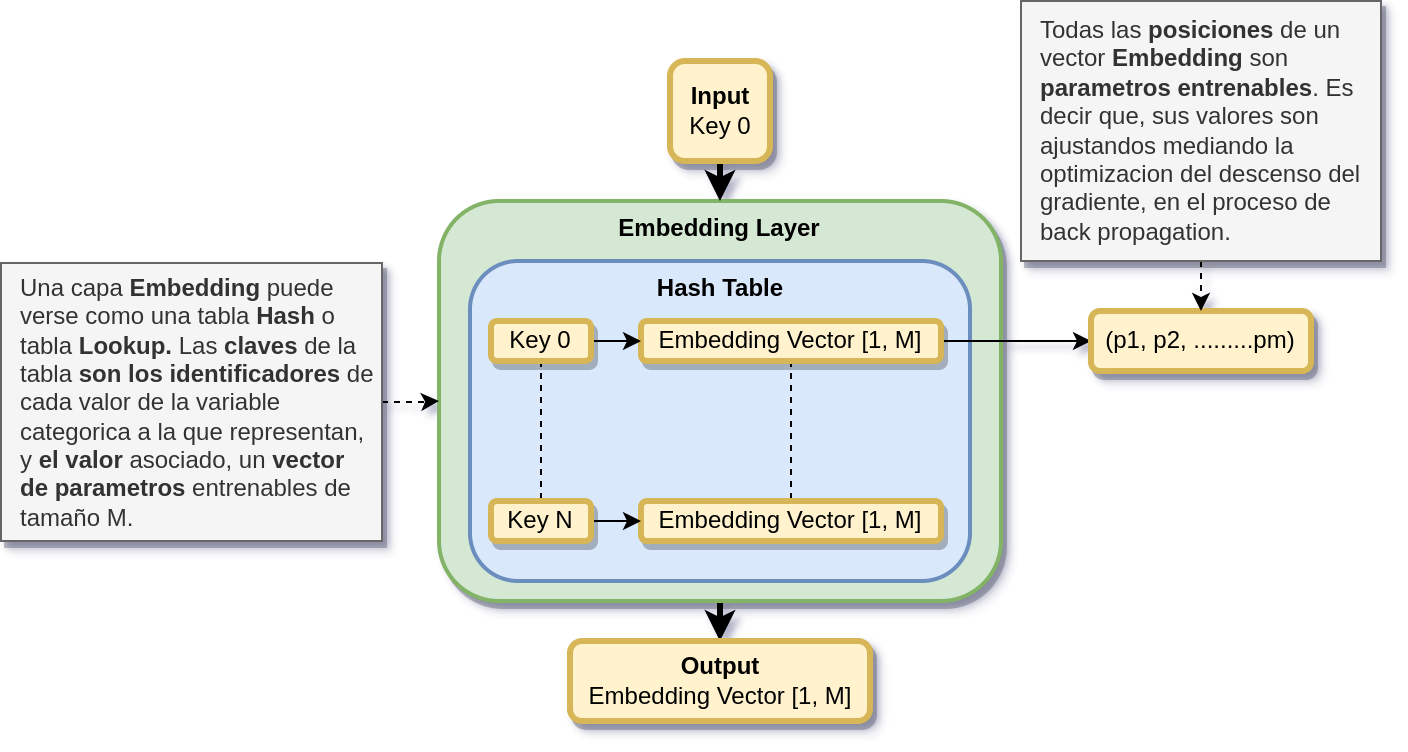
\includegraphics[width=13cm]{./images/Embedding-Layer.png}
\end{center}

Finamente, tengamos en cuenta que el proceso de back-propagation sera encargado de ir ajustando los valores o también llamados pesos de los vectores \textit{embedding} de cuerdo a lo que requiera en la salida del modelos durante el proceso de optimización de descenso del gradiente. 


\subsection{Arquitecturas Utilizadas}

En el apartado anterior se explicó uno de las componente básicos y mas usando en modelos de recomendación basados en modelo de Deep Learning. Des de qui se describirán las arquitecturas utilizadas en este trabajo.

\subsection{General Matrix Factorization (GMF)}

Esta es una arquitectura clásica en sistemas de recomendación basados en filtros colaborativos. El \href{https://sifter.org/~simon/journal/20061211.html}{algoritmo de factorización de matrices} funciona desacoplando la matriz de interacciones usuario-item en un producto escalar de dos matrices regulares de baja dimensionalidad. Este algoritmo o familia de algoritmos fue popularizado por primera por \textit{Simon Funk} en la competencia \href{https://en.wikipedia.org/wiki/Netflix_Prize}{\textit{Netflix prize}} en 2006. La idea principal del algoritmo es representar a usuario e items en un espacio latente de baja dimensionalidad.
A partir del trabajo inicial realizado por  \textit{Funk} en 2006, se han propuesto multiples enfoque de factorización de matrices para sistemas de recomendación, siento este el modelo de mas simple y efectivo.

Este modelo se puede construir fácilmente realizando el producto escalar de dos matrices de vectores de \textit{embeddings}, las cuales tiene una baja dimensionalidad debido al principio de funcionamiento de los \textit{embeddings}. A continuación se puede ver un esquema del modelo, el cual toma como entradas los identificadores de un usuario e item, luego resuelven los vectores \textit{embedding} correspondiente a ambos ids, y finalmente se realiza el producto escalar de ambos vectores. Este producto escalar da como resultado la calificación del usuario para el item dado. Por otro lado, el algoritmo del optimización de gradiente descendente sera quien se ocupe de ajustar los pesos de ambas matrices para que dado un id de usuario y otro id de item se obtenga la calificación correspondiente a la observación utilizada como ejemplo de entrenamiento.

\begin{center}
	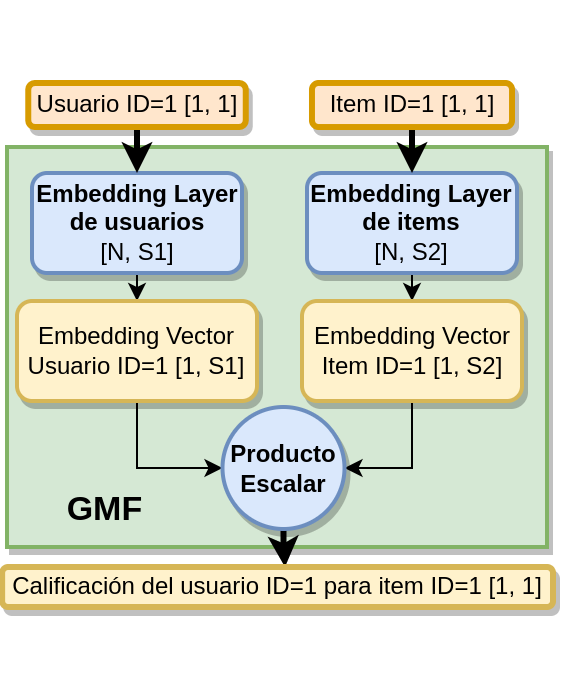
\includegraphics[width=6cm]{./images/GMF.png}
\end{center}

En términos matemáticos este modelo realiza la siguiente operación, en cada paso hacia adelante (\textit{forward-pass}):

\begin{equation*}
	\tilde{r}_{u, i} = V_u . V_i^{T}
\end{equation*}
\begin{description}
	\item[Donde:]
\end{description}
\begin{itemize}
	\item $V_u$ es el vector \textit{embedding} correspondiente al usuario $u$.
	\item $V_i^{T}$ el vector \textit{embedding} correspondiente al item $i$.
	\item $ \tilde{r}_{u, i}$ es la predicción de la calificación realizada por el usuario $u$ al item $i$ (Valor escalar).
\end{itemize}

En términos matriciales podemos verlo de la siguiente manera:

\begin{equation*}
	\tilde{R} = U.I
\end{equation*}
\begin{description}
	\item[Donde:]
\end{description}
\begin{itemize}
	\item $U\in\mathbb{R}^{u \times f}$ es la matriz de vectores \textit{embedding} de usuarios, la cual tiene tantas filas $u$ como usuarios y el la dimensión del numero de columnas (también llamada factor latente) corresponde al tamaño seleccionado para los vectores \textit{embedding}. 
	\item $I\in\mathbb{R}^{f\times items}$ es la matriz de vectores \textit{embeddings} de items, la cual tiene tantas filas como factores latente en los vectores \textit{embedding}, y tantas columnas como items se tenga. 
	\item $\tilde{R}\in\mathbb{R}^{usuarios \times items}$ es la matriz de calificaciones, donde cada fila corresponde a un usuario y columna a un item.
\end{itemize}


El tamaño de la dimensión de factores latentes como ya se vio anteriormente en el apartado \textit{One-Hot vs. Embeddings} es un hiper-parámetro mas a ajustar. \href{https://link.springer.com/chapter/10.1007/978-3-642-38844-6_3}{Se ha demostrado} que realizar factorización de matrices con un factor latente de tamaño 1 es equivalente a un modelo de recomendación por popularidad, es decir que recomienda los items mas populares sin tener en cuenta la personalización de las recomendaciones. Luego, a medida que vamos incrementando el tamaño del factor latente estar recomendaciones serán cada ves mas personalizadas aumentando la calidad de las mismas. Cuando el tamaño del factor latente es muy grande, el modelos comienza a sobre ajustar(overfitting) y por ende la calidad de las recomendaciones comentara a empeorar. Para solucionar este se suelen agregar términos de regularización en la función de error a minimizar:

\begin{equation*}
\underset{H, W}{\operatorname{arg\,min}}\, \|R - \tilde{R}\|_{\rm F} + \alpha\|H\| + \beta\|W\|
\end{equation*}
\begin{description}
\item[Donde:]
\end{description}
\begin{itemize}
\item $\|.\|_{\rm F}$ se define como [[norma matricial]] mientras que las otras normas pueden ser matricial u otro tipo de normal dependiendo del sistema de recomendación.
\end{itemize}

\subsection{\textit{Biased General Matrix Factorization (B-GMF)}}

El modelo \textit{GMF} de \textit{Simon Funk} realiza recomendaciones de muy buena calidad, pero tiene como limitación que solo utilizar interacciones usuario-item que tiene que ver con valores numéricos referidos a interacciones explicitas como calificaciones. Los sistemas de recomendación modernos deben explotar todas las interacciones posibles, tanto explícitas (Calificaciones numéricas) como implícitas (Me gusta, Compras, Vistas, Favoritos, etc..). Para solucionar este nuevo problema donde es necesario usar cualquier tipo de interacción usuario item explicita o implícita se agrega un Bias o sesgo para los usuarios y otro para los items.

A Continuación se puede aprecia el diagrama del modelo, muy similar al diagrama anterior:

\begin{center}
	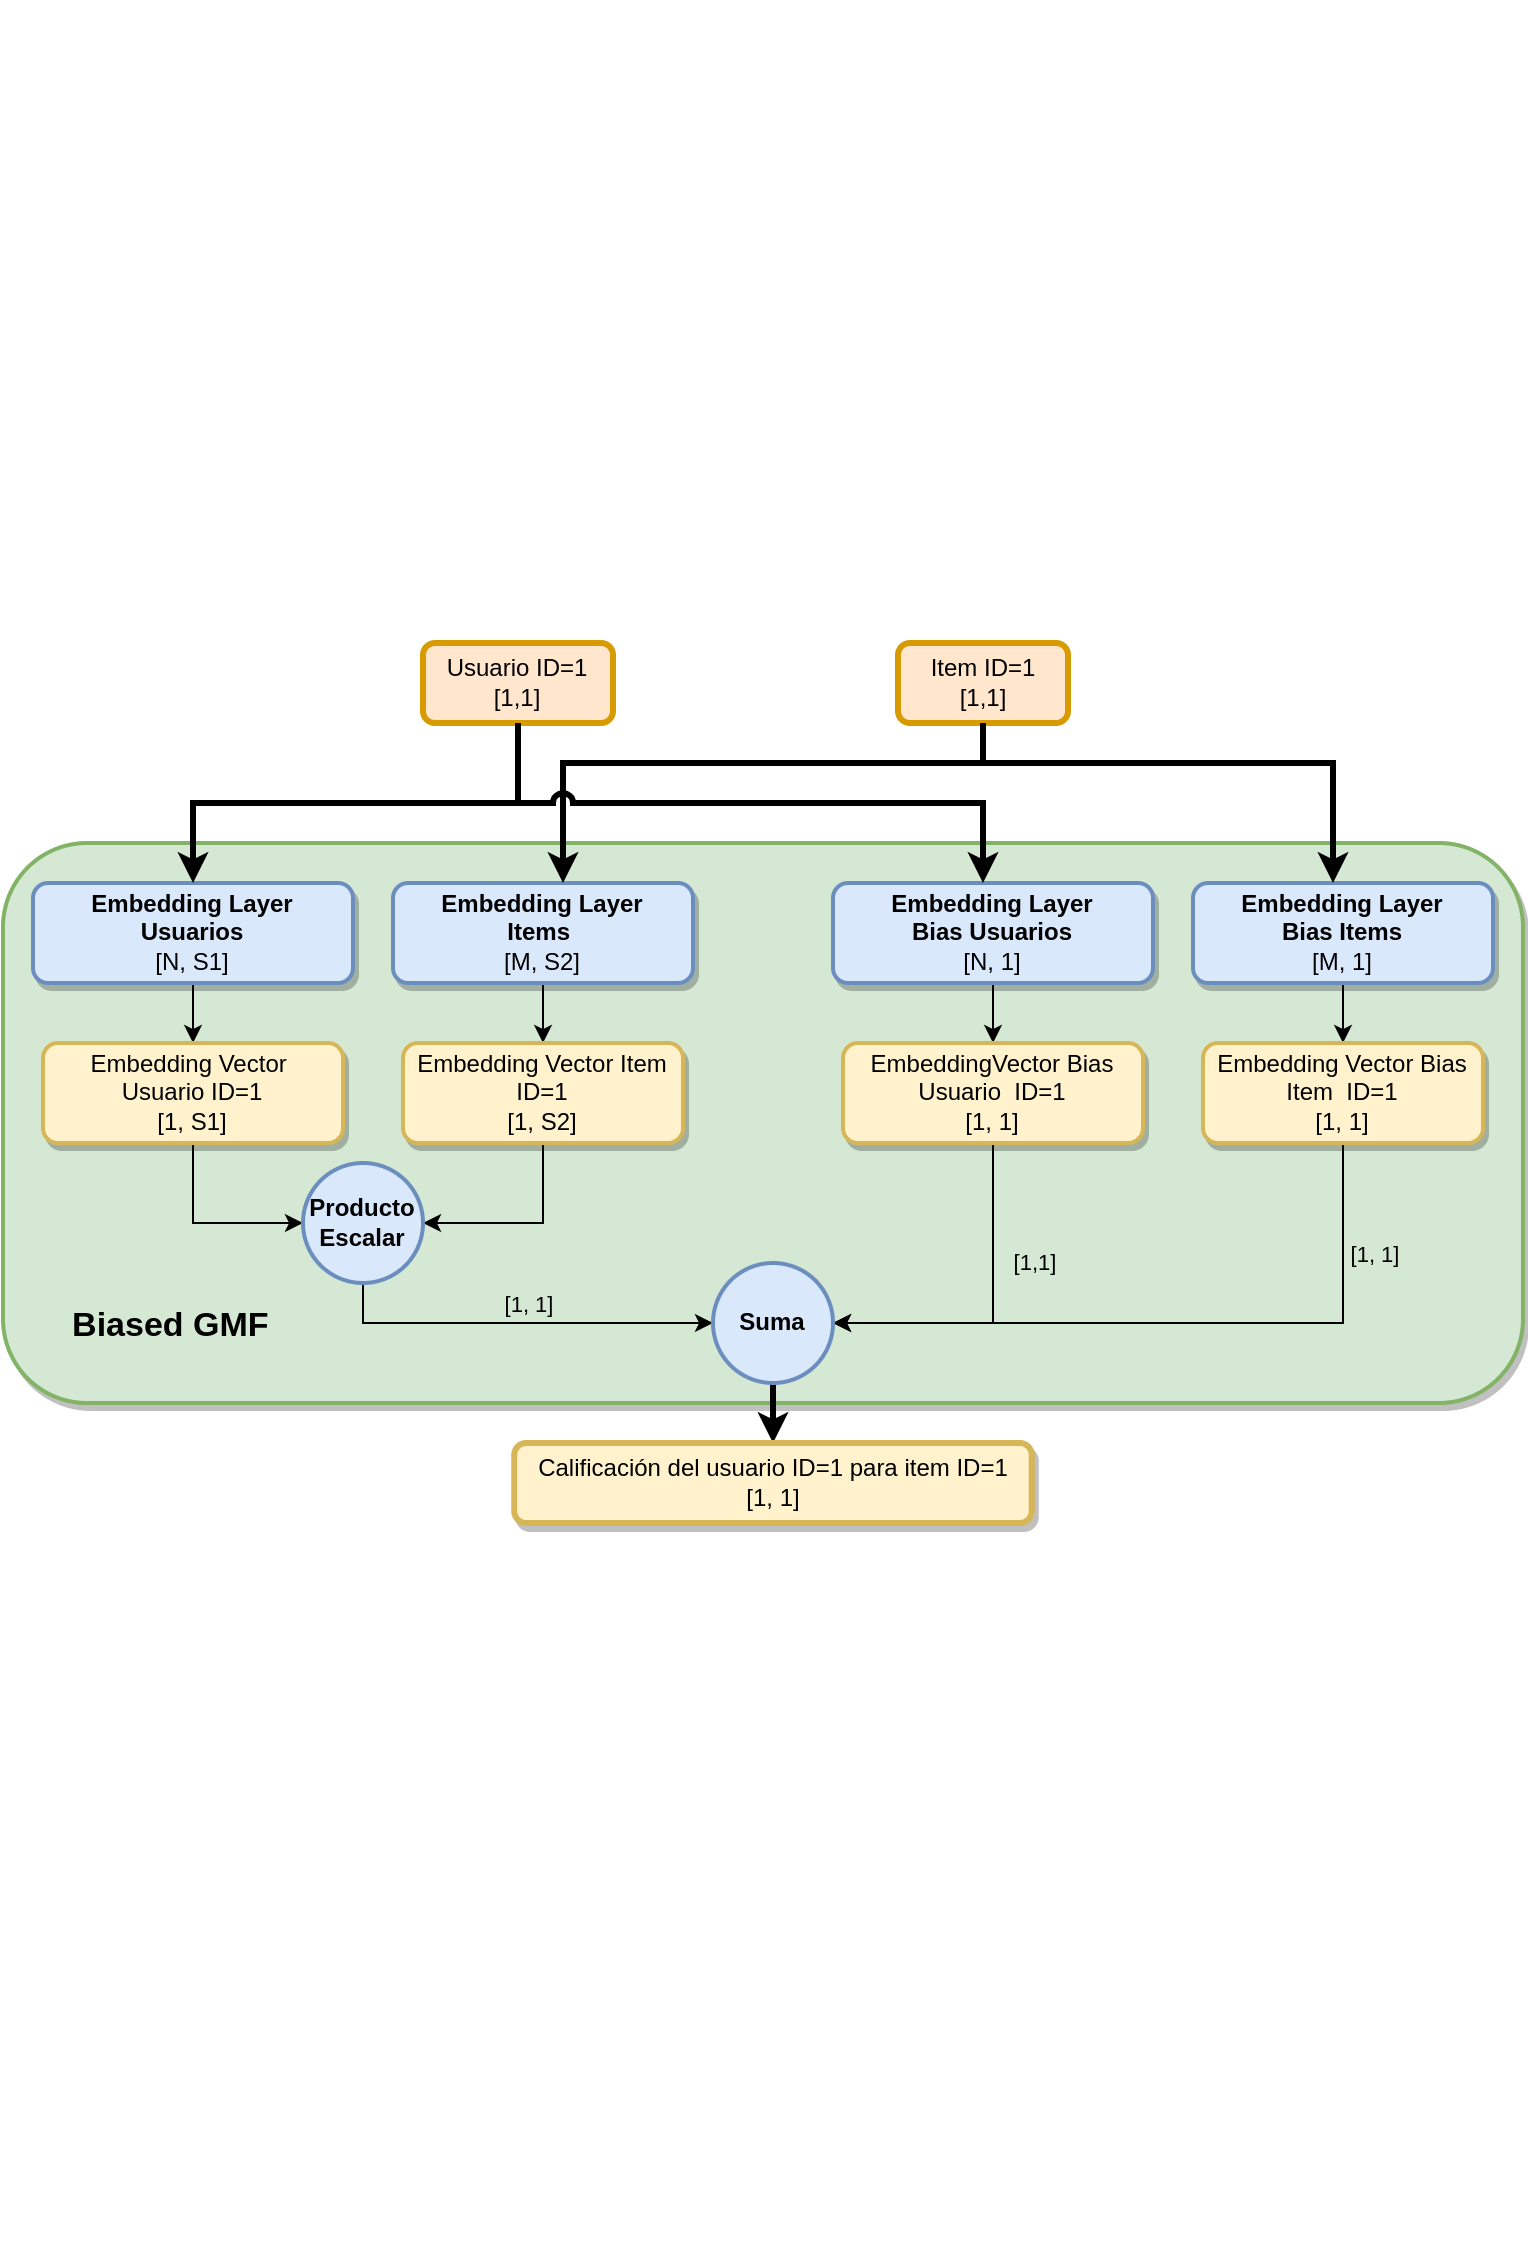
\includegraphics[width=11cm]{./images/Biased-GMF.png}
\end{center}

En este caso se agregan dos nuevas \textit{Embedding Layers}, las cuales representa a los sesgos de usuarios e items respectivamente. El tamaño de los factores latentes o vectores \textit{embedding} correspondiente a cada \textit{bias} es 1, es decir son valores escalares. Finalmente, luego de calcular el producto escalar se suman los factores latentes resultado de ambas \textit{Embedding Layers} correspondiente a los biases.  


\subsection{\textit{Neural Network Matrix Factorization (NN-MF)}}

Con los enfoques anteriormente vistos (\textit{GFM} y \textit{Biased GFM}) dada dos matrices de baja dimensionalidad se realiza un producto escalar y se suman sesgos dependiendo de caso para calcular o inferir la calificación del usuario para un item dado. Estos modelos como ya se conto aprender los pesos o parámetros de los vectores \textit{embeddings} en el proceso se entrenamiento. 

El enfoque de \href{https://arxiv.org/pdf/1511.06443.pdf}{\textit{Neural Network Matrix Factorization (NN MF)}} es levemente distinto. En este caso se reemplaza el producto interno, el cual podemos pensarlo como conocimiento a priori del problema, por otra función desconocida que sera la que aprenderá el modelo a partir de las observaciones suministradas en su entrenamiento. En particular se remplaza el producto escalar mas los sesgos por una red neuronal multi capa de capas densas o fully connected. De esta forma, el modelo no solo aprender los parámetros de los vectores \textit{embedding}, sino también los pesos de la red multi capa y en definitiva cual es la mejor función para predecir las calificaciones del usuario, como cualquier otro tipo de interacción.

Utilizar rede neuronales abre el panorama, ya que ahora podemos usar mas variable que sea relevante a nuestro problema de predicción y no solo las variable categóricas y usuario e items; aquí es donde recibe el mayor potencial de este enfoque.

a continuación podemos ver un esquema del modelo, muy similar a \textit{GFM} como ya se dijo, con la diferencia que tenemos una red multi capa en vez de un producto escalar.

\begin{center}
	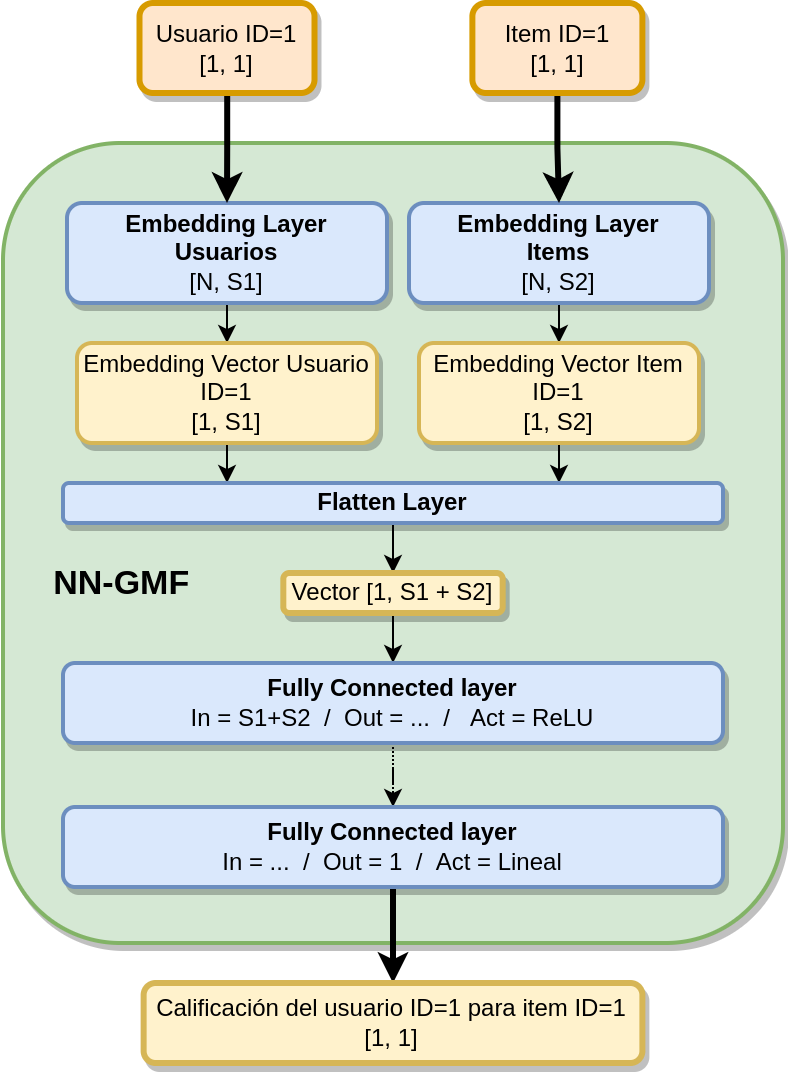
\includegraphics[width=6cm]{./images/NN-MF.png}
\end{center}


Entonces, como entradas tenemos los identificadores de usuarios e items en entradas independientes (Escalares). Cone sto identificadores cada \textit{Embedding Layer} resuelve el vector \textit{embedding} asociado. Acto siguiente el bloque \textit{Flatter} toma ambos vectores y devuelve un nuevo vector el cual es la concatenación de los do anteriores. En el siguiente paso este nuevo vector es al entrada de la red multi capa, es decir que la red multi capa tendrá tanta entradas como posiciones tenga este vector. La cantidad de capas y neuronas por capas de la red so hiper-parámetros vana  ir cambiando en el proceso de optimización de hiper-parámetros, pro esa cuestión no se especifican un numero de capas. Cada capa menos la ultima tiene una función de activación ReLU y la ultima capa por supuesto un activación \textit{Lineal} al igual que una regresión lineal, ya que queremos predecir las calificaciones que tienen un rango de valores reales entre 0.5 y 5. Cave aclarar que se esta pensando como segundo enfoque usar una activación \textit{Softmax} en vez de una \textit{Lineal} en la ultima capa. De esta manera, se podría abordar como un problema de clasificación ya que los valores de las calificaciones son números reales pero también son discretos.


\subsection{Factorization Machines (FM)}


Antes de introducir el modelo \textit{Deep Factorization Machine} vamos a comenzar explicando un de lso componente principales de este: Las \textit{Máquinas de factorización}. 

Las \href{https://www.csie.ntu.edu.tw/~b97053/paper/Rendle2010FM.pdf}{Maquinas de Factorización} propuestas por \textit{Steffen Rendle} en 2010,son algoritmos supervisados que se puede utilizar para tareas de clasificación, regresión y tareas de ranking como sucede en el ámbito de recomendaciones. Rápidamente se convivieron en un método popular para hacer predicciones y recomendaciones. La \textit{Máquina de factorización} es una generalización de un modelo lineal y un model de factorización de matrices, mas aun, recuerdan mucho a un \textit{Maquina de soporte vectorial(SVM)} que utiliza un kernel polinomial.

F
Formalmente, si tenemos:

\begin{itemize}
	\item $x\in\mathbb{R}^{d}$ es un vector de features donde cada una de sus componentes representa a una variable del \textit{dataset}, siendo $d$ la cantidad de variables de \textit{dataset¨} (excluyendo la columna de labels). En nuestro caso $x\in\mathbb{R}^{2}$ ya que tenemos dos variables, usuarios e items.
	\item $y\in\mathbb{R}$ es la variable target a predecir, en nuestro caso es la calificación del usuario. 
\end{itemize}

podemos definir el modelo para una \textit{máquina de factorización} de grado dos de ls siguiente forma:

\begin{equation*}
\hat{y}(x) = \mathbf{w}_0 + \sum_{i=1}^d \mathbf{w}_i x_i + \sum_{i=1}^d\sum_{j=i+1}^d \langle\mathbf{v}_i, \mathbf{v}_j\rangle x_i x_j
\end{equation*}
\begin{description}
	\item[Donde:]
\end{description}
\begin{itemize}
	\item $\mathbf{w}_0 \in \mathbb{R}$ es el bias global.
	\item $\mathbf{w} \in \mathbb{R}^d$ es el peso asociado a la variable $i^\mathrm{th}$.
	\item $\mathbf{V} \in \mathbb{R}^{d\times k}$ representa a un vector \textit{embedding} asociado al la variable $i^\mathrm{th}$.
	\item $\mathbf{v}_i$ representa a la $i^\mathrm{th}$ fila de la matriz $\mathbf{V}$. 
	\item $k$ es la dimensionalidad del factor latente o tamaño de lso vectores \textit{embedding}.
	\item $\langle\cdot, \cdot \rangle$ es el producto interno de dos vectores.
	\item $\langle \mathbf{v}_i, \mathbf{v}_j \rangle$ modelos la interacción entre $i^\mathrm{th}$ y $j^\mathrm{th}$ variable. 
\end{itemize}

De esta forma los dos primeros términos corresponden al modelo de regresión lineal y el último término es una extensión del modelo de factorización matricial. Si la variable $i$ representa un item y la variable $j$ a un usuario, el tercer término es el producto escalar entre los vectores \textit{embedding} de usuario $u$ y item $i$. Por otro lado, vale la pena aclarar que este método también puede generalizar en órdenes superiores al grado 2, sin embargo, la estabilidad numérica podría disminuí la generalización del método.


Al aplicar un método de optimización con las máquinas de factorización, como puede el método del gradiente descendente, se puede llegar fácilmente a una complejidad del orden $\mathcal{O}(kd^2)$, ya que se deben calcular todas las interacciones de a pares. Para resolver este problema de insuficiencia, podemos reorganizar el tercer término del método, lo que podría reducir en gran medida el costo de cálculo, lo que lleva a una complejidad de tiempo de orden lineal $\mathcal{O}(kd)$. A continuación se describe los pasas para bajar el nivel de complejidad del método:


\begin{equation*}
\begin{split}
&=\sum_{i=1}^d \sum_{j=i+1}^d \langle\mathbf{v}_i, \mathbf{v}_j\rangle x_i x_j \\
&= \frac{1}{2} \sum_{i=1}^d \sum_{j=1}^d\langle\mathbf{v}_i, \mathbf{v}_j\rangle x_i x_j - \frac{1}{2}\sum_{i=1}^d \langle\mathbf{v}_i, \mathbf{v}_i\rangle x_i x_i \\
&= \frac{1}{2} \big (\sum_{i=1}^d \sum_{j=1}^d \sum_{l=1}^k\mathbf{v}_{i, l} \mathbf{v}_{j, l} x_i x_j - \sum_{i=1}^d \sum_{l=1}^k \mathbf{v}_{i, l} \mathbf{v}_{i, l} x_i x_i \big)\\
&=  \frac{1}{2} \sum_{l=1}^k \big ((\sum_{i=1}^d \mathbf{v}_{i, l} x_i) (\sum_{j=1}^d \mathbf{v}_{j, l}x_j) - \sum_{i=1}^d \mathbf{v}_{i, l}^2 x_i^2 \big ) \\
&= \frac{1}{2} \sum_{l=1}^k \big ((\sum_{i=1}^d \mathbf{v}_{i, l} x_i)^2 - \sum_{i=1}^d \mathbf{v}_{i, l}^2 x_i^2)
\end{split}
\end{equation*}

Con esta re-formulación de último termino, la complejidad del método se reduce considerablemente. Además, para las variables ralas, solo se deben computar los valores distintos de cero para que la complejidad general sea lineal. Finalmente la expresión del método aplicada esta re-formulación queda como sigue:

\begin{equation*}
	\hat{y}(x) = \mathbf{w}_0 + \sum_{i=1}^d \mathbf{w}_i x_i + \frac{1}{2} \sum_{l=1}^k \big ((\sum_{i=1}^d \mathbf{v}_{i, l} x_i)^2 - \sum_{i=1}^d \mathbf{v}_{i, l}^2 x_i^2)
\end{equation*}


\subsection{\textit{Deep Factorization Machine (DeepFM)}}

Hasta aquí, a grandes rasgos, todo los modelos vistos tratan de captar el comportamiento de las interacciones o correlación usuario-items ya sean implícita o explicitas. A pesar de este gran progreso, los métodos expuestos anteriormente(exceptuando las \textit{Máquinas de Factorización}) parecen tener un fuerte sesgo al predecir las interacciones o correlaciones de bajo y alto orden, requiriendo en algunos casos realizar ingeniería de features para disminuir estos sesgos. 

El modelo \href{https://arxiv.org/pdf/1703.04247.pdf}{\textit{Deep Factorization Machine (DeepFM)}} o Maquina de factorización basada en \textit{Deep Learning}, mejora el aprendizaje de las interacciones o correlaciones de bajo y alto orden. Este modelo combina \textit{Máquinas de Factorización} y \textit{Deep Learning} en una nueva arquitectura de red neuronal la cual captura estas correlaciones. Por otro lado, es una evolución del modelo \href{https://arxiv.org/pdf/1606.07792.pdf}{Wide and Deep} de Google, el cual es un ensample de dos modelos: uno lineal, que captura las interacciones o correlaciones de alto orden y una MLP (Multi-Layer Perceptron) la cual captura correlación de mas bajo orden, o aquellas mas complejas.

A continuación de puede visualizar un diagrama de bloques de alto nivel de modelos:

\begin{center}
	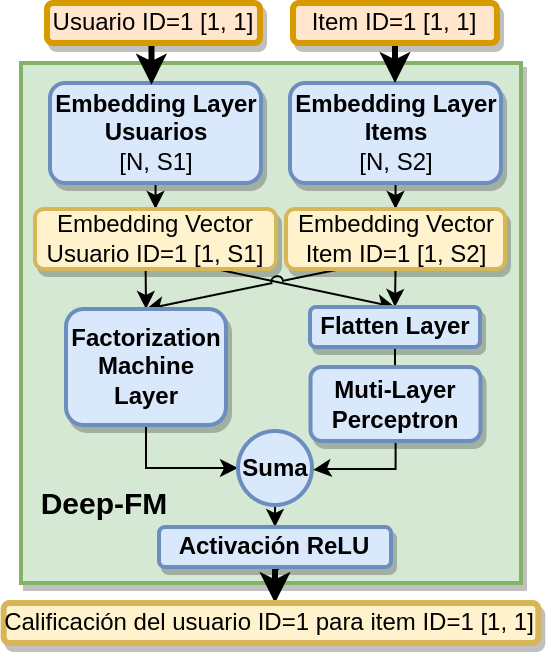
\includegraphics[width=6cm]{./images/Deep-MF.png}
\end{center}

Donde se puede apreciar que las entradas del modelo son las variables categóricas correspondiente a usuarios e items, como en los modelos previamente visto.
dado un id de usuario y item se resuelve sus correspondientes vectores \textit{embedding}, los cuales se convierten en entradas para los siguientes dos bloques. Uno de los bloques no es mas que una red neuronal multi capa con capas densa o fully connected. Por el otro lado ambos vectores se toman como entrada a la \textit{maquina de factorización}. las salida de ambos bloques son volares escalares los cuales se suman y se pasan por una activación \textit{ReLU} ya que en nuestro caso las calificaciones son valores mayos a cero.


\section{Métricas}

Pra medir y comparar el grado de exactitude de los modelos seleccionados tanto en el conjunto de validación como en truncamiento se seleccionado dos métricas:

\begin{itemize}
	\item \textit{Root Mean Square Error (RMSE)}: ES la raíz cuadrada del error cuadrático medio.
	\item \textit{Mean Average Precision at k (mAP@k)}: Es la media del promedio de la precision  para un tamaño K de observaciones.
\end{itemize}

\subsection{\textit{Root Mean Square Error (RMSE)}}

Dado que todos los modelo se evaluaron en este trabajo tiene como salida una variable real (Calificación de los usuarios para un item), es posible utilizar \textit{RMSE}, la cual es  
utilizada en problemas de regresión donde la salida del modelo es una variable numérica real.

Si bien esta métrica no es la métrica por excelencia a usar en el ámbito de sistemas de recomendación, ayuda a comprender cuales el grado de ajuste de los modelos y pue servir como una métrica complementara al momento de evaluar los mismos.

\begin{description}
	\item[Definición:]
\end{description}
\begin{equation*}
	\operatorname{RMSE}=\sqrt{  \frac{1}{N} \sum_{i=1}^N (y_i - \hat y_i)^2}
\end{equation*}
\begin{description}
	\item[Donde:]
\end{description}
\begin{itemize}
	\item $y_i$ es el true value o verdad de campo de la observación.
	\item $\hat y_i$ es la predicción realizada por el modelo predictor.
	\item $N$ es el numero de observaciones sobre las que se realizo la predicción del modelo.
\end{itemize}

\subsection{\textit{Mean Average Precision at k (mAP@k)}}

\textit{Mean Average Precision at k (mAP@k)} o media del promedió de la precision para K observaciones, es una de las métricas mas usada para evaluar sistemas de recomendación.

Si pensamos a nivel de aplicación de un sistemas de recomendación pedimos ver entras y salidas donde:


\begin{itemize}
\item Entradas: Como entradas tenemos el identificador del usuario al cual queremos presentarle recomendaciones y otro parámetro opcional que podría ser el identificador de un item. ¿Por que opcional? Bueno, en general si no especificamos un id de item, es posible encontrar cuales son lo items de mayor preferencia para el usuario y luego recomendar nuevos items en base a este item inicial. Por otro lado, si ya se cuenta con un id de item, se puede recomendar item similares en este. Este ultimo caso es muy común cuando un usuario navega al detalle de un producto en un e-commerce, en este punto ya se conoce el id del usuario y id de item. Finalmente se recomienda items similares al item visualizado.
\item Salidas: Es una lista de items recomendados similares a otro item (Entrada del modelo) ordenado descendentemente por la calificación predicha por el modelo para el usuario en cuestión(Entrada del modelo). 
\end{itemize}


De esta forma, al encontrar en las primeras posiciones de la lista, aquellos items que tiene la calificación predicha mas alta, es un indicado de que el modelo es preciso al momento de recomendar. En palabras mas simples, se desea que los primeros items de la lista de recomendaciones sean de mayor agrado para el usuario.

¿Finalmente, como funciona esta métricas?

La métrica \textit{mAP\makeatletter@k} funciona de la siguiente forma:

Supongamos que tenemos un usuario y una lista K de item a recomendar. En base a estas entadas el modelo de recomendación predice las calificaciones de cada item para el usuario dado. Luego. podemos ordenar la lista de item descendentemente de acuerdo a las calificaciones predicha por el modelo.

Teniendo esta lista se puede calcular el promedio de la perdición \textit{mAP\makeatletter@k} sobre los K items de la lista.

Esta métricas es utilizada en problema de clasificación pero también se puede utilizar en problemas donde el modelo produce una salida numérica com en este caso. Los niveles o clases a utilizar dependen mucho de que se quiera evaluar. Supongamos, en este caso particular, que queremos medir con que precisión las puntuaciones entre 4 y 5 aparecen en las primera posiciones de la lista, para esto usaremos la métricas \textit{mAP\makeatletter@k}.

\begin{description}
	\item[Promedio de la precisión sobre una lista de K elementos \textit{AP\makeatletter@k}):]
\end{description}
\begin{equation*}
	\begin{split}
	& \operatorname{AP\makeatletter@k}=\frac{1}{N(k)} \sum_{i=1}^k \frac{ TP(i)}{i}, \\
	& \\
	& \operatorname{N(k)} = min(k, TP_{total}) \\
	\end{split}
\end{equation*}
\begin{description}
	\item[Donde:]
\end{description}
\begin{itemize}
	\item $TP_i$ es 1 si la precision y el valor verdadero concuerdan.
	\item $i$ es la posición del item $i^\mathrm{th}$ en la lista de $k$ elementos.
	\item $N(k)$ es el mínimo entre el tamaño de la lista y la cantidad de $TP_{total}$ encontrados en esa lista.
\end{itemize}

Por ejemplo si queremos saber con que precision aparecen en las primeras posiciones de la lista de $k$ elementos items con calificaciones entre 4 y 5 puntos, podemos pensar que un $TP_i == 1$ o verdadero, si la calificación en la posición $i^\mathrm{th}$ se encuentra entre los 4 y 5 punto, caso contrario $TP_i == 0$. De esta forma transformar la salida del modelo en clase binarias para utilizar métrica.

A continuación se calcula resta calicular \textit{AP\makeatletter@k} para cada usuario  del \textit{dataset} de validación y finalmente se calcula media: 


\begin{description}
	\item[Media del promedio de la precisión sobre una lista de K elementos \textit{mAP\makeatletter@k}):]
\end{description}
\begin{equation*}
	\operatorname{mAP\makeatletter@k}=\frac{1}{N} \sum_{i=1}^N AP\makeatletter@k_i
\end{equation*}

De esta forma, la métricas \textit{AP\makeatletter@k} nos da una noción del grado de precisión en que aparecen items con mayor puntuación en las primeras posiciones de una lista de tamaño $k$.


\chapter{Experimentos}

Para compara todos modelos implementados, se utilizo el mismo \textit{dataset}, tomando una muestra con el tamaño suficiente para obtener buenos resultado, evitando el sobre ajuste(overfitting) para aquellos modelos que tienden a sobre ajustar mas. Por otro lado, se realizaron optimización en el modelo \textit{KNN} para poder cachear resaltados y de esta forma no repetir predicciones al momento de samplear muestra del conjuntos de validación.

Por otro lado, cabe aclarar que dada la tendencia de los modelos a la variabilidad o varianza de sus predicciones, se realizo un sampleo de cada métrica sobre el conjunto de validación N veces. Luego, se gráfico un histograma de la distribución de la métricas y un boxplot para tener una mejor idea de cual es su valor medio de la misma y que dispersion se puede esperar.


A continuación se describen los resultados de todos los modelos comparados mediando las métricas \textit{AP\makeatletter@k} y \textit{RMSE}.

\section{\textit{K-Nearest-Neighbor (KNN)}}

\subsection{\textit{KNN Item Based}}

\begin{figure}[!htb]
	\centering
	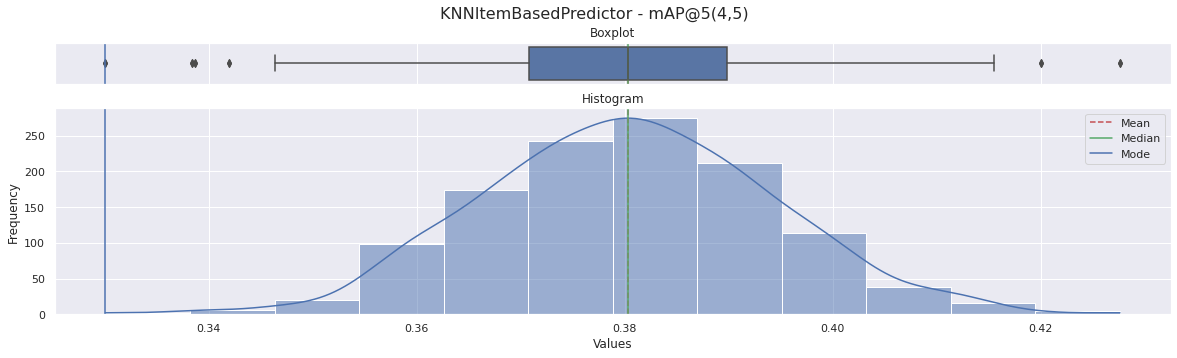
\includegraphics[width=15cm]{./images/metrics-knn-item-based-mapk.png}
	\caption{Esta gráfica describe un histograma del valor de la métrica \textit{mAP@5(4,5)} evaluado en el conjunto de observaciones de validación, luego de N procesos de entrenamiento del modelo \textit{KNN Item Based} sobre las observaciones de entrenamiento.}
\end{figure}

\clearpage


\begin{figure}[!htb]
	\centering
	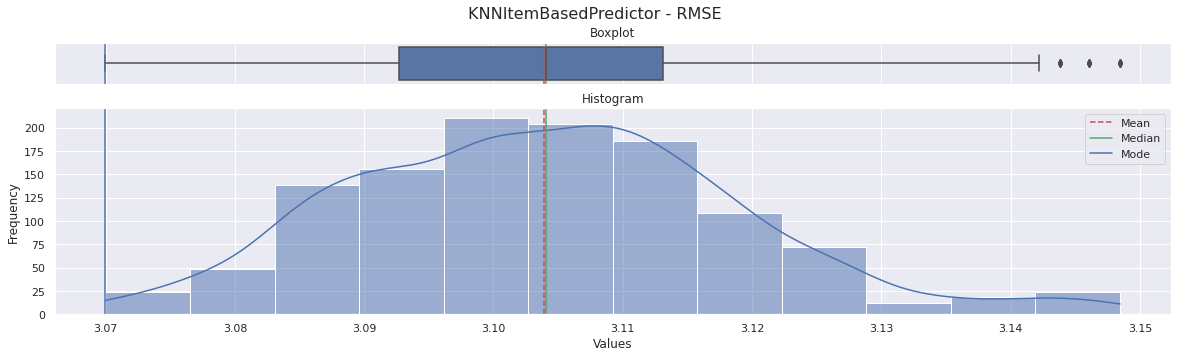
\includegraphics[width=15cm]{./images/metrics-knn-item-based-RMSE.png}
	\caption{Esta gráfica describe un histograma del valor de la métrica \textit{RMSE} evaluado en el conjunto de observaciones de validación, luego de N procesos de entrenamiento del modelo \textit{KNN Item Based} sobre las observaciones de entrenamiento.}
\end{figure}

\subsection{\textit{KNN User Based}}

\begin{figure}[!htb]
	\centering
	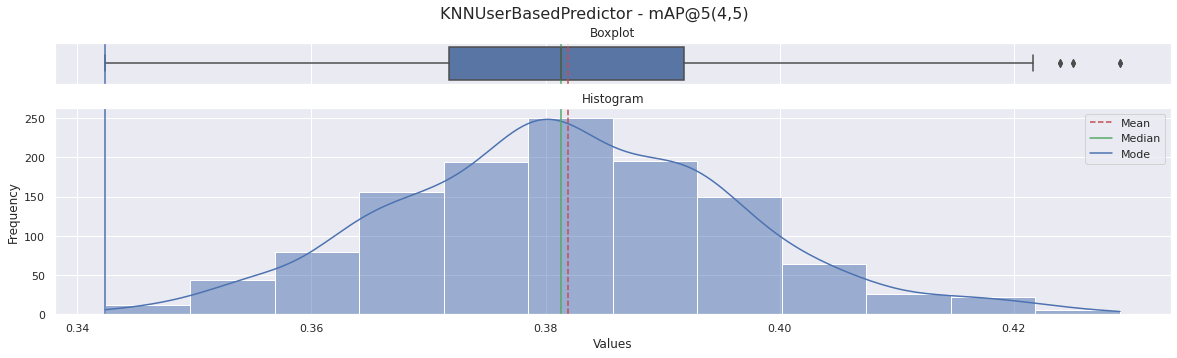
\includegraphics[width=15cm]{./images/metrics-knn-user-based-mapk.png}
	\caption{Esta gráfica describe un histograma del valor de la métrica \textit{mAP@5(4,5)} evaluado en el conjunto de observaciones de validación, luego de N procesos de entrenamiento del modelo \textit{KNN User Based} sobre las observaciones de entrenamiento.}
\end{figure}


\begin{figure}[!htb]
	\centering
	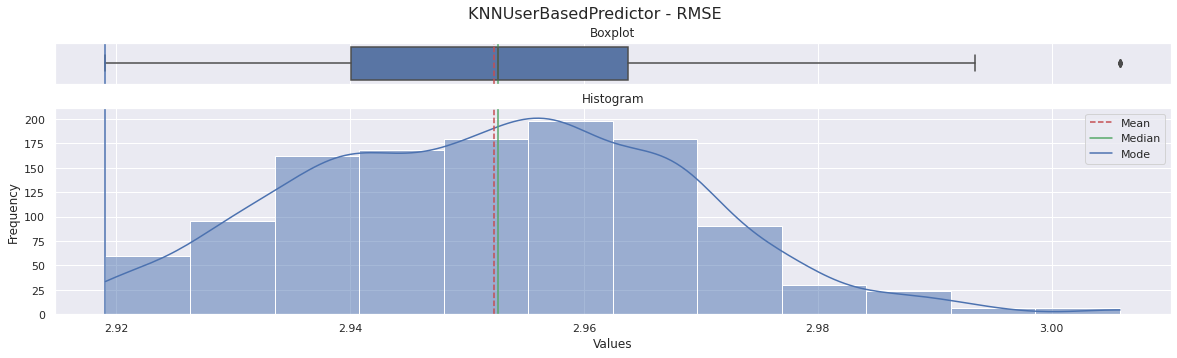
\includegraphics[width=15cm]{./images/metrics-knn-user-based-RMSE.png}
	\caption{Esta gráfica describe un histograma del valor de la métrica \textit{RMSE} evaluado en el conjunto de observaciones de validación, luego de N procesos de entrenamiento del modelo \textit{KNN User Based} sobre las observaciones de entrenamiento.}
\end{figure}



\clearpage

\subsection{\textit{Ensample KNN User Based} y \textit{Item Based}}

\begin{figure}[!htb]
	\centering
	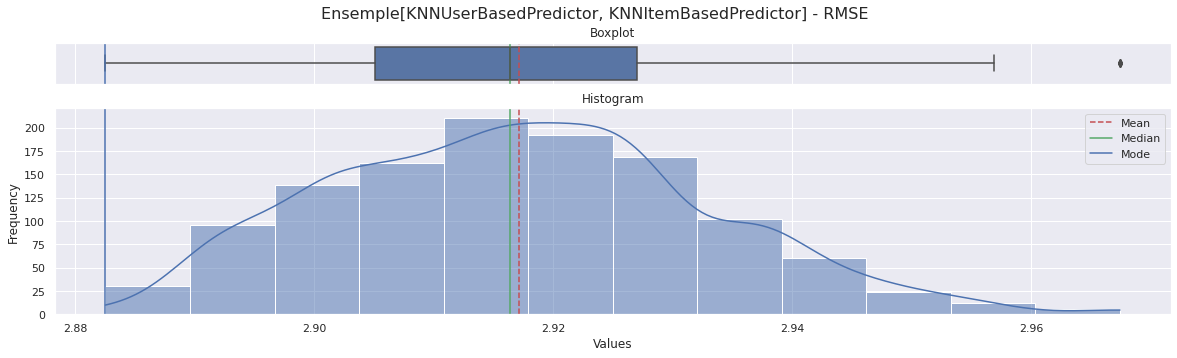
\includegraphics[width=15cm]{./images/metrics-knn-ensemple-RMSE.png}
	\caption{Esta gráfica describe un histograma del valor de la métrica \textit{RMSE} evaluado en el conjunto de observaciones de validación, luego de N procesos de entrenamiento del modelo \textit{KNN} sobre las observaciones de entrenamiento.}
\end{figure}

\begin{figure}[!htb]
	\centering
	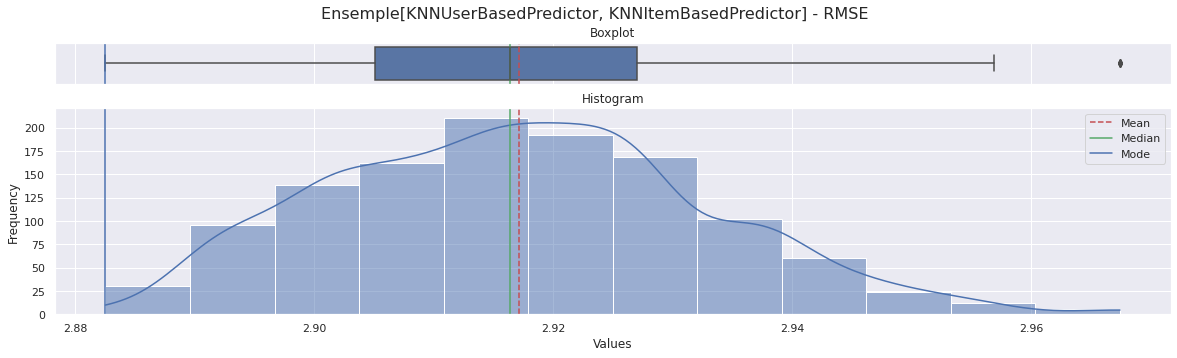
\includegraphics[width=15cm]{./images/metrics-knn-ensemple-RMSE.png}
	\caption{Esta gráfica describe un histograma del valor de la métrica \textit{RMSE} evaluado en el conjunto de observaciones de validación, luego de N procesos de entrenamiento del modelo \textit{KNN} sobre las observaciones de entrenamiento.}
\end{figure}


\clearpage
\section{\textit{General Matrix Factorization (GFM)}}

A continuación se puede apreciar las cursas de la $Loss$ (\textit{MSE}) para el conjunto de validación y entrenamiento:

\begin{figure}[ht]
	\centering
	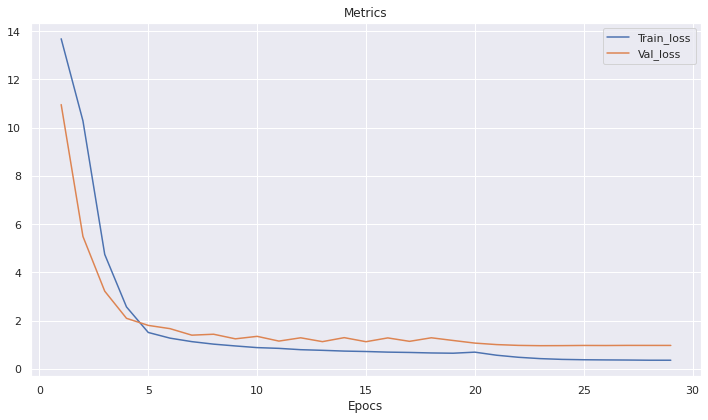
\includegraphics[width=13cm]{./images/metrics-GFM-train-val-loss.png}
	\caption{Esta gráfica describe el nivel de error sobre los conjuntos de observaciones de entrenamiento y validación durante el entrenamiento del modelo \textit{GFM}. Cada epoch o época indica una iteración de entrenamiento del modelo sobre el conjunto completo de entrenamiento.}
\end{figure}

Se puede apreciar que inicialmente el modelo tiene un error de valoración menor al error de entrenamiento. Es posible que se deba a que una pocas primeras observaciones de entrenamiento fueron suficientes para predecir con un error menor el conjunto de validación. A media que se incrementa el numero de épocas ya no es subiente y el modelo comienza a sobre ajusta hasta estabilizarse ambos errores.


\clearpage

\begin{figure}[h!]
	\centering
	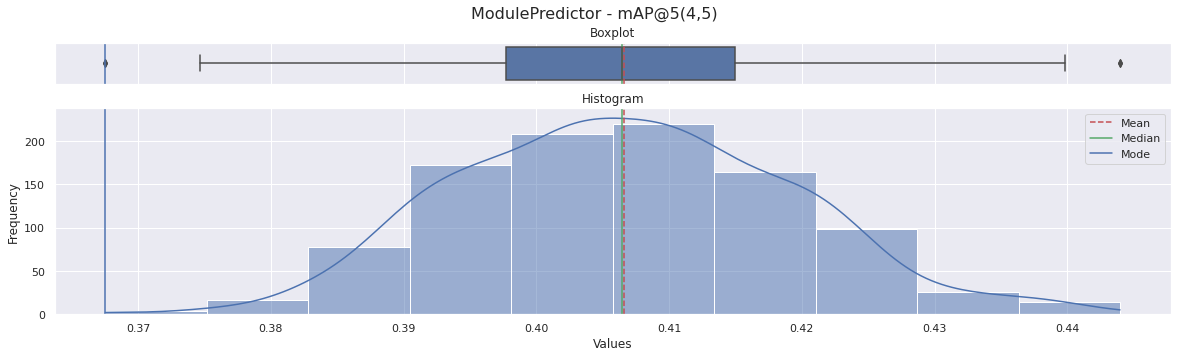
\includegraphics[width=15cm]{./images/metrics-GFM-mapk.png}
	\caption{Esta gráfica describe un histograma del valor de la métrica \textit{mAP@5(4,5)} evaluado en el conjunto de observaciones de validación, luego de N procesos de entrenamiento del modelo \textit{GFM} sobre las observaciones de entrenamiento.}
\end{figure}

Dado la tendencia de los modelos a la variabilidad o varianza de sus predicciones se realizo un sampleo de cada métrica sobre el conjunto de validación N veces para comprender cual es su valor medio y dispersión.

\begin{figure}[h!]
	\centering
	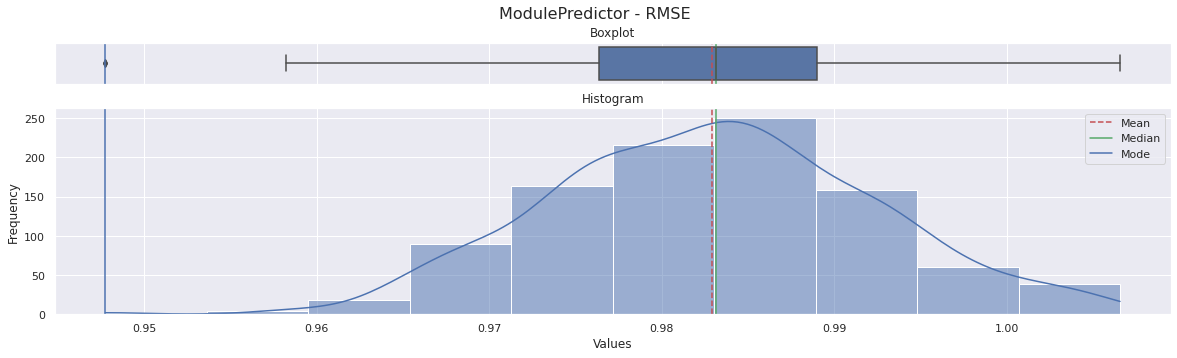
\includegraphics[width=15cm]{./images/metrics-GFM-RMSE.png}
	\caption{Esta gráfica describe un histograma del valor de la métrica \textit{RMSE} evaluado en el conjunto de observaciones de validación, luego de N procesos de entrenamiento del modelo \textit{GFM} sobre las observaciones de entrenamiento.}
\end{figure}



\clearpage
\section{\textit{Biased General Matrix Factorization (B-GFM)}}

\begin{figure}[h!]
	\centering
	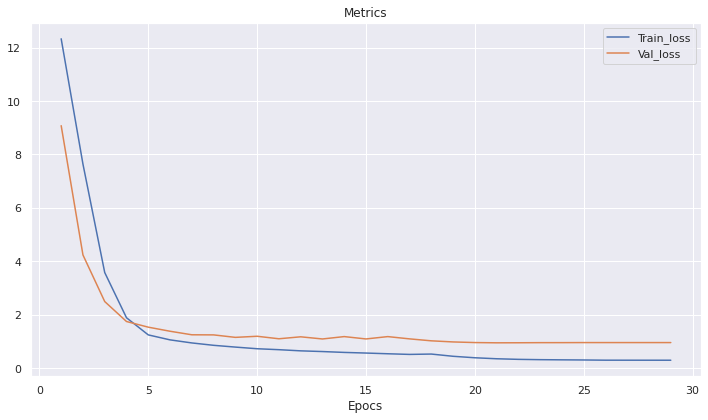
\includegraphics[width=13cm]{./images/metrics-BGFM-train-val-loss.png}
	\caption{Esta gráfica describe el nivel de error sobre los conjuntos de observaciones de entrenamiento y validación durante el entrenamiento del modelo \textit{B-GFM}. Cada epoch o época indica una iteración de entrenamiento del modelo sobre el conjunto completo de entrenamiento.}
\end{figure}

\begin{figure}[h!]
	\centering
	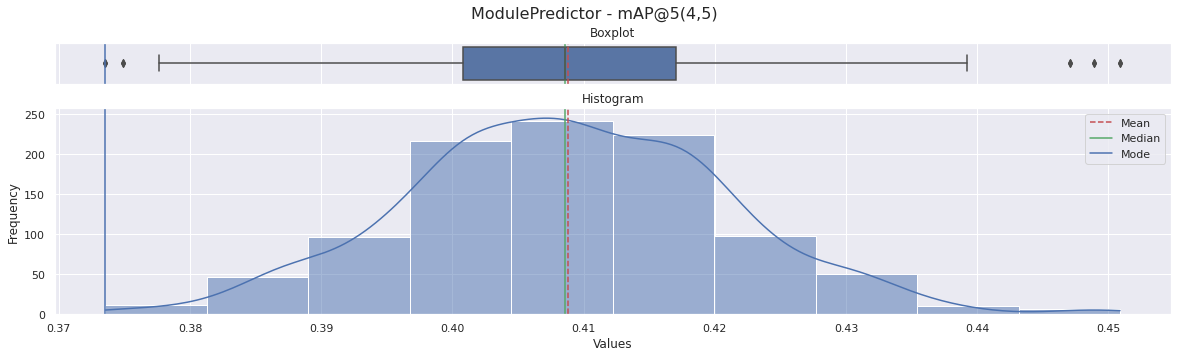
\includegraphics[width=15cm]{./images/metrics-BGFM-mapk.png}
	\caption{Esta gráfica describe un histograma del valor de la métrica \textit{mAP@5(4,5)} evaluado en el conjunto de observaciones de validación, luego de N procesos de entrenamiento del modelo \textit{B-GFM} sobre las observaciones de entrenamiento.}
\end{figure}


\clearpage

\begin{figure}[h!]
	\centering
	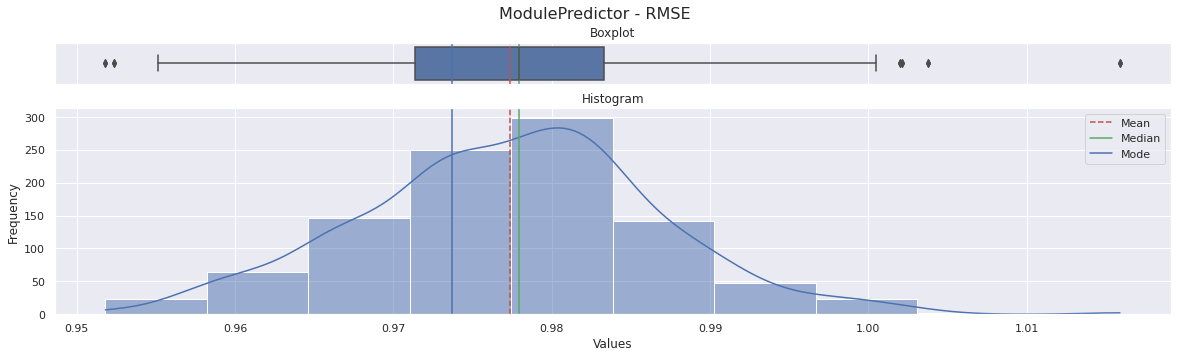
\includegraphics[width=15cm]{./images/metrics-BGFM-RMSE.png}
	\caption{Esta gráfica describe un histograma del valor de la métrica \textit{RMSE} evaluado en el conjunto de observaciones de validación, luego de N procesos de entrenamiento del modelo \textit{B-GFM} sobre las observaciones de entrenamiento.}
\end{figure}




\section{Neural Network Matrix Factorization (NN-FM)}

\begin{figure}[h!]
	\centering
	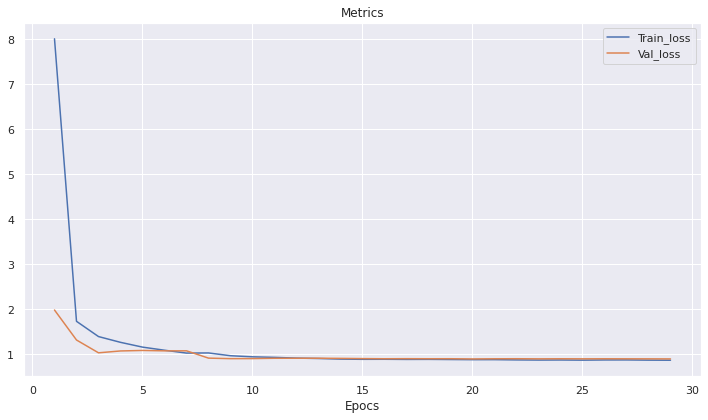
\includegraphics[width=13cm]{./images/metrics-NN-FM-train-val-loss.png}
	\caption{Esta gráfica describe el nivel de error sobre los conjuntos de observaciones de entrenamiento y validación durante el entrenamiento del modelo \textit{NN-FM}. Cada epoch o época indica una iteración de entrenamiento del modelo sobre el conjunto completo de entrenamiento.}
\end{figure}


\clearpage

\begin{figure}[h!]
	\centering
	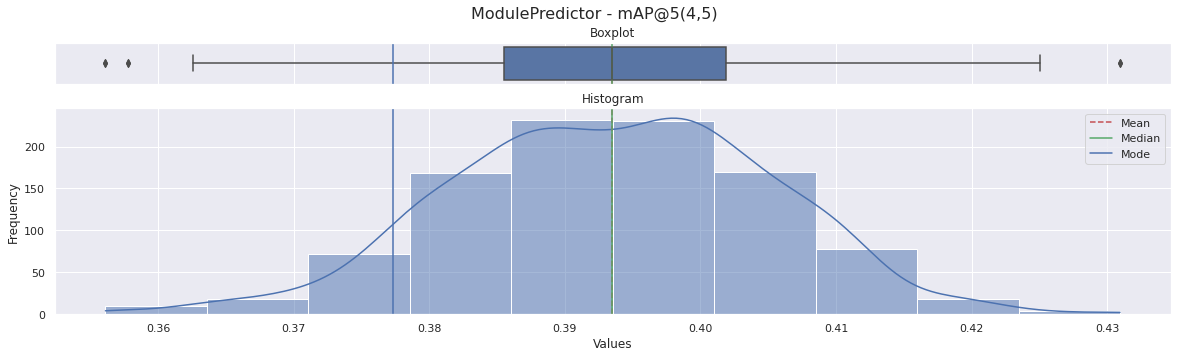
\includegraphics[width=15cm]{./images/metrics-NN-FM-mapk.png}
	\caption{Esta gráfica describe un histograma del valor de la métrica \textit{mAP@5(4,5)} evaluado en el conjunto de observaciones de validación, luego de N procesos de entrenamiento del modelo \textit{NN-FM} sobre las observaciones de entrenamiento.}
\end{figure}

\begin{figure}[h!]
	\centering
	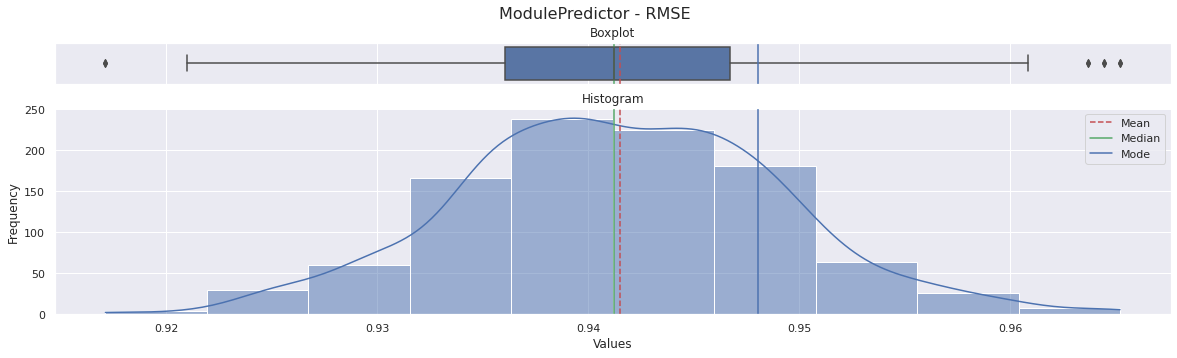
\includegraphics[width=15cm]{./images/metrics-NN-FM-RMSE.png}
	\caption{Esta gráfica describe un histograma del valor de la métrica \textit{RMSE} evaluado en el conjunto de observaciones de validación, luego de N procesos de entrenamiento del modelo \textit{NN-FM} sobre las observaciones de entrenamiento.}
\end{figure}




\clearpage

\section{\textit{Deep Factorization Machine (DeepFM)}}

\begin{figure}[h!]
	\centering
	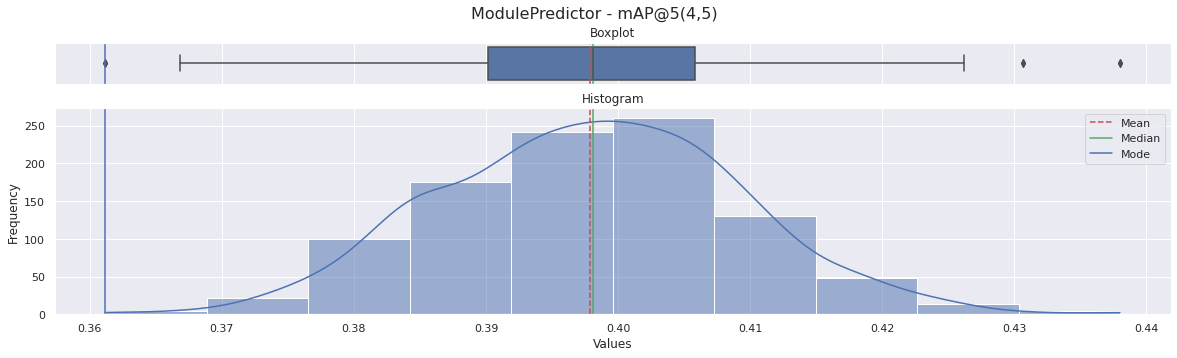
\includegraphics[width=15cm]{./images/metrics-DeepFM-mapk.png}
	\caption{Esta gráfica describe un histograma del valor de la métrica \textit{mAP@5(4,5)} evaluado en el conjunto de observaciones de validación, luego de N procesos de entrenamiento del modelo \textit{DeepFM} sobre las observaciones de entrenamiento.}
\end{figure}

\begin{figure}[h!]
	\centering
	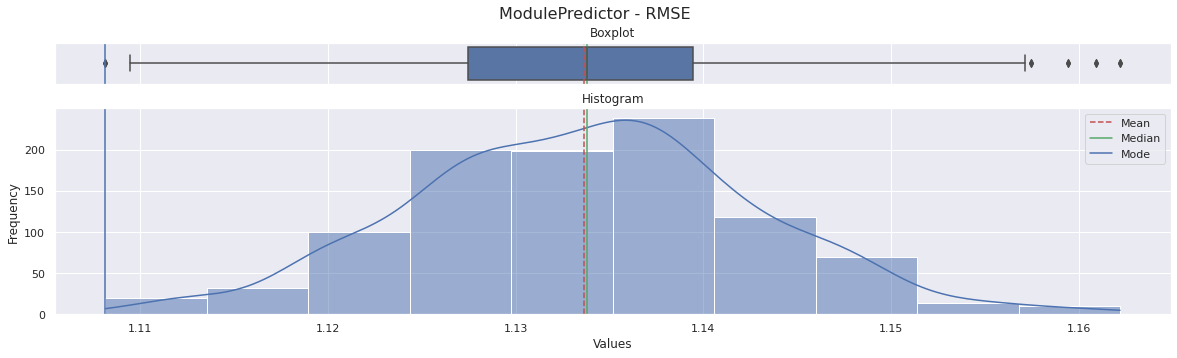
\includegraphics[width=15cm]{./images/metrics-DeepFM-RMSE.png}
	\caption{Esta gráfica describe un histograma del valor de la métrica \textit{RMSE} evaluado en el conjunto de observaciones de validación, luego de N procesos de entrenamiento del modelo \textit{DeepFM} sobre las observaciones de entrenamiento.}
\end{figure}



\chapter{Resultados}

A continuación se muestra una tabla comparativa con las métricas utilizadas para todos los modelos:

\begin{table}[!htb]
	\centering
	\footnotesize
	\begin{tabular}{lrrr}
	\hline
		Modelo                       & Mediana  & Media    & Desvio  \\
	\hline
	\textit{B-GMF}                        & 0.408563 & 0.408787 & 0.012190 \\
	\textit{GMF¨}                          & 0.406422 & 0.406646 & 0.012513 \\
	\textit{DeepFM}                       & 0.398100 & 0.397895 & 0.011369 \\
	\textit{NN-MF}                        & 0.393499 & 0.393447 & 0.011711 \\
	\textit{KNN User-Item Based Ensemble} & 0.384570 & 0.384819 & 0.015066 \\
	\textit{KNN User Based}               & 0.381297 & 0.381943 & 0.014709 \\
	\textit{KNN Item Based}               & 0.380284 & 0.380327 & 0.014056 \\
	\hline
	\end{tabular}
	\caption{
		Mediana, Media y Desvío correspondientes a las distribución de 
		\textit{AP\makeatletter@5(4,5)} sampleada para cada modelo. Las filas se encuentran ordenadas descendentemente por la Media.
	}
	\label{table:tab}
\end{table}


\begin{description}
	\item[Observaciones:]
\end{description}
\begin{itemize}
\item A primera vista se aprecia Biased-GMF es el modelo con mejores resultados con la métricas de evaluación \textit{AP\makeatletter@5(4,5)}.
\item Por otro lado, podemos ver que los modelos \textit{NN-MF} y \textit{Deep-FM} tiene el menor sesgo, pero aun asi tiene precisiones menores al modelo \textit{Biased-GMF}. Esto podría indicar un grado mayor de sobre ajuste. por ende, se debería re-entrenar los modelos \textit{NN-MF} y \textit{Deep-FM} aumentando el dropout para mejorar la regularización y volver a compara contra \textit{Biased-GMF} para validar si las precisiones mejoran.
\item La familia de modelos \textit{KNN} son lo que presentan mayor sesgo en la precision. A pesar de esto podemos ver que la diferencia de precision con los demás de modelos es muy baja, mejor al 2 \%.
\end{itemize}


\begin{table}[!htb]
	\centering
	\footnotesize
	\begin{tabular}{lrrr}
		\hline
			Modelo                       & Mediana  & Media    & Desvio  \\
		\hline
		\textit{NN-MF}                        & 0.941213 & 0.941493 & 0.007620 \\
		\textit{B-GMF}                        & 0.977914 & 0.977382 & 0.009387 \\
		\textit{GMF}                          & 0.983141 & 0.982894 & 0.009419 \\
		\textit{DeepFM}                       & 1.133796 & 1.133637 & 0.009183 \\
		\textit{KNN User-Item Based Ensemble} & 2.916418 & 2.917146 & 0.015642 \\
		\textit{KNN User Based}               & 2.952661 & 2.952305 & 0.016170 \\
		\textit{KNN Item Based}               & 3.104068 & 3.103917 & 0.014975 \\
		\hline
	\end{tabular}
	\caption{
		Mediana, Media y Desvío correspondientes a las distribución de 
		\textit{RMSE} sampleada para cada modelo. Las filas se encuentran ordenadas  descendentemente por la Media.
	}
	\label{table:tab}
\end{table}

\begin{description}
	\item[Observaciones:]
\end{description}
\begin{itemize}
\item A simple vista \textit{NN-MF} es el modelo mas estable en cuando al error de validación, ya que tiene el menor error y dispersion. aun asi no es el modelo pas preciso. Esto podría indicar que tiene un grade de sobre ajuste major a modelos con mayor precision.
\item Podemos apreciar que el modelo \textit{Biased-GMF} con mayor precision aui tiene un error mayor a \textit{NN-MF}. OIndicando que la teoría del sobre ajuste de \textit{NN-MF} podría ser valida.
\item Nuevamente la familia de modelos \textit{KNN} tiene los errores mas alto y también altos desvíos. Aun asi estos modelos tiene una precisión muy similar al modelo mas preciso (\textit{B-GMF}).
\end{itemize}


\chapter{Conclusiones}

Como conclusiones, se puede decir que no se encuentra una gran diferencia en precisión entre todos modelos, siendo esta menor al 2 \%. Por otro lado, si tuviésemos que llevar alguno de esto modelos a producción e un e-commerce, claramente se elegiría un modelo basado en \textit{deep learning}, como pueden ser \textit{B-GMF} o \textit{GMF}. Esto se debe a que estos modelos utilizan el algoritmo del gradiente descendente, pudiendo procesar las observaciones de entrenamiento en lotes. De esta forma, se puede seleccionar un tamaño de lote que se ajuste a la memoria \textit{RAM} o \textit{VRAM} disponible. Por lo contrario no seria posible selecciona modelos de la familia \textit{KNN} debido a que necesitan alocar todas las observaciones den entrenamiento en memoria.

Por otro lado, podemos apreciar que un modelo en el estado de arte como \textit{DeepFM}, no obtiene la precision mas alta, e inclusive su precisión es prácticamente igual a las precisiones obtenidas por la familia de modelo \textit{KNN}.
Finalmente podemos decir que en el caso de estas pruebas el \textit{dataset} utilizado, los modelo de \textit{deep learning} obtienen mejores resultado que modelos mas clásicos como \textit{KNN}, pero estos resultados son muy similares.


%%%% BIBLIOGRAFÍA
\backmatter
%\bibliography{tesis}

\end{document}
